\documentclass[a4paper, oneside, openany, dvipsnames, table, 12pt]{article}
\usepackage{../../../Template/AFKstyle}
\usepackage{hyperref}
\usepackage{verbatim} %per commenti di più righe \begin{comment} \end{comment}
\usepackage{amsmath}
\newcommand{\Titolo}{Verbale interno 2020-06-05}

\newcommand{\Gruppo}{TeamAFK}

\newcommand{\Redattori}{}

\newcommand{\Verificatori}{}

\newcommand{\pathimg}{../../../../Template/img/logoAFK.png}

\newcommand{\Approvatore}{}

\newcommand{\Distribuzione}{Prof. Vardanega Tullio \newline Prof. Cardin Riccardo \newline TeamAFK}

\newcommand{\Uso}{Interno}

\newcommand{\NomeProgetto}{"Predire in Grafana"}

\newcommand{\Mail}{gruppoafk15@gmail.com}

\newcommand{\Versionedoc}{1.0.0}

\newcommand{\DescrizioneDoc}{Riassunto dell'incontro del gruppo \textit{TeamAFK} tenutosi il 2020-06-05.}


\makeindex

%------------------ PER SISTEMARE INDICE TABELLE E FIGURE 
\makeatletter
\renewcommand*\l@figure{\@dottedtocline{1}{1.5em}{3em}}% 3em instead of 2.3em
\let\l@table\l@figure
\makeatother
%------------------

\begin{document}
\copertina{}

%------------------ COLORI TABELLE 
\definecolor{pari}{RGB}{255, 207, 158} %{HTML}{E1F5FE} %azzurrino
\definecolor{dispari}{HTML}{FAFAFA} %bianco/grigetto 

%definizione colori per tabelle (tranne copertina)
\definecolor{redafk}{RGB}{255, 133, 51}
\definecolor{grey2}{RGB}{204, 204, 204}
\definecolor{greyRowafk}{RGB}{234, 234, 234}
\definecolor{lastrowcolor}{RGB}{176, 196, 222} %steel blue %{255,165,0} orange %{RGB}{255, 207, 158}
\rowcolors{2}{pari}{dispari}
\renewcommand{\arraystretch}{1.5}

%------------------

\newpage
\section*{Registro delle modifiche}
{
	\centering
	\begin{longtable}{ c c  C{4cm}  C{4cm}  C{3cm} }
		\rowcolor{redafk}
		\textcolor{white}{\textbf{Versione}} & \textcolor{white}{\textbf{Data}} & \textcolor{white}{\textbf{Descrizione}} & \textcolor{white}{\textbf{Nominativo}} & \textcolor{white}{\textbf{Ruolo}}\\		
		2.1.1 & 2020-05-27 & Aggiunta incrementi \S 6.2. Verificato il documento. & &\adm{} \newline \ver{} \\
		2.1.0 & 2020-05-26 & Refactoring \S 4.1 e \S 4.3. Apportate modifiche normative al \textit{Registro delle Modifiche}. Verificato il documento. & Davide Zilio \newline Victor Dutca & \adm{} \newline \ver{} \\
		2.0.0 & 2020-05-10 & Approvazione del documento per la RP. & Davide Zilio &\RdP{} \\
		1.1.0 & 2020-05-08 & Stesura \S 6.2. Verificato il documento. & Simone Meneghin \newline Alessandro Canesso &\adm{} \newline \ver{}\\
		1.0.2 & 2020-05-06 & Ampliamento \S 2. Verificato il documento. & Victor Dutca \newline Alessandro Canesso &\Res{} \newline \ver{}\\
		1.0.1 & 2020-04-30 & Correzioni e stesura \S 2.1. Verificato il documento. & Simone Meneghin \newline Alessandro Canesso &\Res{} \newline \ver{}\\
		1.0.0 & 2020-04-12 & Approvazione del documento per la RR. & Victor Dutca &\RdP{} \\
		0.7.0 & 2020-03-10 & Stesura \S B. Verificato il documento. & Alessandro Canesso \newline Olivier Utshudi &\Res{} \newline \ver{}\\
		0.6.0 & 2020-03-10 & Stesura \S 6. Verificato il documento. & Alessandro Canesso \newline Olivier Utshudi &\Res{} \newline \ver{}\\
		0.5.0 & 2020-03-06 & Stesura \S 5. Verificato il documento.  & Fouad Farid \newline Olivier Utshudi &\Res{} \newline \ver{}\\
		0.4.0 & 2020-04-04 & Stesura \S 4. Verificato il documento. & Simone Federico Bergamin \newline Simone Meneghin &\adm{} \newline \ver{}\\	
		0.3.0 & 2020-04-03 & Stesura \S 3. Verificato il documento.  & Simone Federico Bergamin \newline Olivier Utshudi &\adm{} \newline \ver{}\\	
		0.2.0 & 2020-03-30 & Stesura \S 2. Verificato il documento.  & Alessandro Canesso \newline Simone Meneghin &\Res{} \newline \ver{}\\	
		0.1.0 & 2020-03-30 & Stesura \S 1. Verificato il documento. & Alessandro Canesso \newline Simone Meneghin &\Res{} \newline \ver{}\\		
	\end{longtable}
} 


%Didascalia tabelle/immagini (prendono come riferimento la subsection)
\counterwithin{table}{subsection}
\counterwithin{figure}{subsection}
\newpage

%indice, indice figure e indice tabelle
\tableofcontents
\newpage
\listoffigures
\newpage
\listoftables
\newpage

\begin{comment}

ATTENZIONE
1) all'inizio e fino a metà maggio tutti hanno più tempo = TUTTI fanno le ore necessarie (base)	
2) le nuove distribuzioni verranno attuate dal 18/05 per le fasi più concitanti del progetto, ossia quelle di:	
- progettazione dettaglio e codifica		
- valutazione e collaudo	
contando che ci saranno da dare tutti, o quasi, gli arretrati da giugno in poi.

NUOVE DISTRIBUZIONI
x = esami arretrati

1) x > 3: -2 ore
2) 2 <= x <= 3: ore base definite per ogni fase
2a) caso Olivier: +1 ora (perchè hai da dare 2(+1) esami (calcolo + RO(+ TW proj)) ma essi sono comunque "meno complicati" di p2 proj e uno tra P3 e algo quindi il tempo da dedicarci è "minore")
3) x < 2: +2 ore

\end{comment}


\section{Introduzione}

\subsection{Scopo del documento}
Il seguente documento ha il compito di stabilire le regole che il team di sviluppo intende seguire in ogni attività di progetto, così da omologare il materiale prodotto.
I fornitori intendono adottare un approccio incrementale\glo, affinché lo sviluppo del prodotto si basi su decisioni prese di comune accordo. Perciò ogni componente del team deve far riferimento a questo documento per garantire la coesione e uniformità delle scelte prese.

\subsection{Scopo del prodotto}
Il capitolato {C4}\glo illustra il prodotto da fornire. Tale prodotto consiste in tool di addestramento ed un plugin\glo di Grafana\glo che prenderà il nome \textit{Predire in Grafana}. Entrambi gli applicativi verranno scritti in linguaggio JavaScript\glo. Il primo avrà il compito di produrre un file di estensione JSON\glo basato su dati di addestramento\glo. Il secondo invece si occuperà di leggere il file creato, effettuare previsioni basandosi su di esso e rendere disponibili al sistema i risultati ottenuti, in modo da poterli visualizzare in grafici e dashboard.
\subsection{Glossario}
Per evitare ambiguità nei documenti formali, viene fornito il documento \textit{Glossario\_v2.0.0}, contenente tutti i termini considerati di difficile comprensione. Perciò nella documentazione fornita ogni vocabolo contenuto in \textit{Glossario\_v2.0.0} è contrassegnato dalla lettera \textit{G} a pedice.
\subsection{Riferimenti}
\subsubsection{Riferimenti normativi}
\begin{itemize}
	\item \textbf{Capitolato d'appalto C4 - Predire in Grafana}: \\
	\url{https://www.math.unipd.it/~tullio/IS-1/2019/Progetto/C4.pdf}.	
\end{itemize}
\subsubsection{Riferimenti informativi}
\begin{itemize}
	\item \textbf{Change Management Process}: \\
	\href{https://www.blog-management.it/2018/04/10/change-management-project-management/}{https://www.blog-management.it/change-management-project-management}\\
	\href{https://www.digital4.biz/hr/hr-transformation/digital-transformation-e-change-management-vanno-avanti-di-pari-passo/}{https://www.digital4.biz/hr/hr-transformation/};
	\item \textbf{The three P's of Software Engineering}: \\
	\url{http://dwaynephillips.net/CutterPapers/ppp/ppp.htm}
	\item \textbf{Software Engineering - Ian Sommerville - 10th Edition}
	\item \textbf{Slide L05 del corso Ingegneria del Software - Ciclo di vita del software}: \\
	\url{https://www.math.unipd.it/~tullio/IS-1/2019/Dispense/L05.pdf};
	\item \textbf{Slide L06 del corso Ingegneria del Software - Gestione di Progetto}: \\
	\url{https://www.math.unipd.it/~tullio/IS-1/2019/Dispense/L06.pdf};	
	\item \textbf{Slide L12 del corso Ingegneria del Software - Qualità di Prodotto}: \\
	\url{https://www.math.unipd.it/~tullio/IS-1/2019/Dispense/L12.pdf};
	\item \textbf{Slide L13 del corso Ingegneria del Software - Qualità di Processo}: \\
	\url{https://www.math.unipd.it/~tullio/IS-1/2019/Dispense/L13.pdf};
\end{itemize}
\pagebreak

\section{Gestione dei rischi}
I rischio viene inteso come l'evento che non vorremmo accadesse nel corso di un progetto, in quanto influenzerebbe in maniera negativa sulla qualità, o sulla riuscita stessa del prodotto. Inoltre, essendo un evento che può riguardare qualunque aspetto del progetto, la gestione dei rischi risulta fondamentale per la riuscita dello stesso. Per questo motivo il gruppo intende affrontare questo compito nel seguente modo:\\
\begin{itemize}
\item \textbf{Identificazione dei rischi}: vengono identificati i rischi, distinguendoli in rischi per il progetto, il prodotto e l'azienda;
\item \textbf{Analisi dei rischi}: viene valutata la probabilità dell'evento e la sua pericolosità;
\item \textbf{Pianificazione dei rischi}: viene stabilito un piano per la prevenzione del rischio annullandone gli effetti, quando possibile, o per lo meno mitigarne le conseguenze;
\item \textbf{Monitoraggio dei rischi}: ad ogni ridefinizione del \textit{Piano di Progetto}, i rischi vengono nuovamente controllati sulla base delle nuove informazioni.
\end{itemize}

\begin{longtable}{C{3cm} L{4.5cm} L{4.5cm} C{3.15cm}}
\rowcolor{white}\caption{Tabella dei rischi} \\
		\rowcolor{redafk}
\textcolor{white}{\textbf{Codice-Nome}} &
\textcolor{white}{\textbf{Descrizione}} &
\textcolor{white}{\textbf{Rilevamento}} &
\textcolor{white}{\textbf{Grado}}  \\
		\endfirsthead
		\rowcolor{white}\caption[]{(continua)} \\
		\rowcolor{redafk}
\textcolor{white}{\textbf{Codice-Nome}} &
\textcolor{white}{\textbf{Descrizione}} &
\textcolor{white}{\textbf{Rilevamento}} &
\textcolor{white}{\textbf{Grado}} \\
		\endhead
		
RiO01 - Emergenza sanitaria &
Un'epidemia riscontrata nel territorio, può costringere le autorità a porre restrizioni per ridurne l'espansione. &
Le restrizioni descritte dal DCPM 2020-03-08 permettono le sole interazioni telematiche tra gli stakeholders. & 
Probabilità: 
Alta 
Pericolosità: 
Alta \\

Piano di contingenza &
\multicolumn{3}{L{13cm}}{Gli stakeholders dovranno decidere di utilizzare gli strumenti di comunicazione disponibili a tutti che limitino i disagi scaturiti dalle suddette restrizioni.} \\

RiT02 - Inesperienza Tecnologica &
Molte delle tecnologie adottate per lo sviluppo del progetto sono nuove per i componenti, che potrebbero usarle in modo non ottimale. &
Il \textit{Responsabile} ha il compito di essere al corrente delle conoscenze dei componenti. & 
Probabilità: 
Alta
Pericolosità: 
Alta\\ 

Piano di contingenza &
\multicolumn{3}{L{13cm}}{Il \textit{Responsabile} una volta messo al corrente delle  conoscenze dei componenti, affiderà loro i ruoli che più li competono.} \\

RiO03 - Calcolo dei costi &
L'insesperienza del gruppo può portare alla sottovalutazione dei costi da sostenere. &
Il \textit{Responsabile} ha il compito di essere al corrente delle conoscenze dei componenti. & 
Probabilità: 
Media 
Pericolosità: 
Alta\\ 

Piano di contingenza &
\multicolumn{3}{L{13cm}}{È consigliato comunicare tempestivamente al committente la variazione dei costi.} \\

RiO04 - Impegni accademici &
Essendo questo un progetto universitario, è probabile che in corso d'opera i componenti debbano sostenere attività accademiche che li sottrarrebbero dagli impegni di progetto. &
Ogni componente deve saper comunicare con chiarezza quelli che sono i propri impegni accademici. & 
Probabilità: 
Alta
Pericolosità: 
Media \\ 

Piano di contingenza &
\multicolumn{3}{L{13cm}}{È consigliato comunicare tempestivamente al \textit{Responsabile} i propri impegni accademici.} \\

RiO05 - Impegni personali &
\'E possibile che in corso d'opera i componeti debbano sostenere attività che li sottrarrebbero, dagli impegni di progetto. &
Ogni componente deve saper comunicare con chiarezza nel calendario quelli che sono i propri impegni. & 
Probabilità: 
Alta
Pericolosità: 
Media \\ 

Piano di contingenza &
\multicolumn{3}{L{13cm}}{È consigliato comunicare tempestivamente al \textit{Responsabile} i propri impegni.} \\


RiO06 - Ritardi &
Le problematiche sopracitate possono comportare ritardi non indifferenti ai fini di progetto. &
Per questo l'incaricato dell'attività deve comunicare tempestivamente il ritardo. & 
Probabilità: 
Media
Pericolosità: 
Bassa \\ 

Piano di contingenza &
\multicolumn{3}{L{13cm}}{È consigliato riassegnare risorse laddove ce ne sia bisogno, e quindi risolvere il motivo del ritardo.} \\

RiP07 - Comunicazione interna &
Può essere che in determinati momenti un elemento del gruppo non sia raggiungibile. &
I membri del gruppo devono segnalare la momentanea assenza dell'interessato/a. & 
Probabilità: 
Bassa
Pericolosità: 
Alta \\ 

Piano di contingenza &
\multicolumn{3}{L{13cm}}{Il gruppo ha adottato diversi mezzi di comunicazione.} \\

RiP08 - Comunicazione esterna &
Se si presentano problematiche come RiO01, il proponente potrebbe non sempre essere reperibile. &
I membri del gruppo organizzeranno le conferenze con il proponente con più largo anticipo. & 
Probabilità: 
Bassa
Pericolosità: 
Alta \\ 

Piano di contingenza &
\multicolumn{3}{L{13cm}}{Il gruppo ha adottato diversi mezzi di comunicazione per rimanere in contatto con il proponente.} \\

RiP09 - Contrasti interni &
Essendo l'attività di progetto un lavoro collaborativo, è possibile che i membri abbiano opinioni divergenti riguardo a determinate tematiche. &
Ciascun membro del team si impegnerà a limitare tali tensioni e fare in modo che esse non influiscano sul normale svolgersi delle attività. & 
Probabilità: 
Bassa
Pericolosità: 
Alta \\ 

Piano di contingenza &
\multicolumn{3}{L{13cm}}{Il responsabile avrà la funzione di gestire e fare da mediatore in tali divergente.} \\

\end{longtable}

\subsection{Attuazione dei rischi}

Nella seguente tabella vengono riportati i rischi in cui il gruppo si è imbattuto:

\begin{table}[H]
\centering\renewcommand{\arraystretch}{1.5}
\caption{Attuazione dei rischi}
\vspace{0.2cm}
\begin{tabular}{ c c c }
\rowcolor{redafk}
\textcolor{white}{\textbf{Rischio}} & \textcolor{white}{\textbf{Descrizione}} & 
\textcolor{white}{\textbf{Contromisura}}  \\
RiO01 - Emergenza sanitaria	& L'epidemia ha costretto a casa gli stakeholders. & Sono stati usati vari mezzi di comunicazione, in particolare si ha optato per applicazioni che permettessero comunicazioni rapide e già conosciute così da ridurre il disagio al minimo.
\\
RiT02 - Inespreienza tecnologica & I programmatori non conoscevano a pieno i linguaggi e le librerie che sono state utilizzate & \'E stato suddiviso il lavoro in modo da rispettare le conoscenze dei membri. In caso di nessuna conoscenza precedente, si è diviso il compito di studiare le documentazioni, per poi spiegarle agli altri membri.
\\
RiO04 - Impegni accademici & Un membro del gruppo ha dovuto svolgere un esame & Durante la breve mancanza di un membro il resto del gruppo si è dedicato all'approfondimento e allo studio delle tecnologie utilizzate
\end{tabular}
\end{table}
\pagebreak

\section{Modello di sviluppo}
Il modello di sviluppo adottato dal gruppo è il \textbf{modello incrementale}.
\subsection{Modello incrementale}
Il modello di sviluppo incrementale vede il progetto come una serie di rilasci (interni e/o esterni), cosicché ad ogni scadenza il materiale consegnato sia sempre più vicino al prodotto finale.
Questo approccio di sviluppo vede la specifica del software, la sua implementazione, convalida ed evoluzione come attività intrecciate tra loro e da sviluppare in parallelo. Quindi il prodotto è considerato tale solo all'ultimo rilascio. Motivo per cui si relaziona bene con il versionamento adottato per il sistema.
L'adozione dello sviluppo incrementale porta i seguenti vantaggi:
\begin{itemize}
\item costi ridotti di implementazione;
\item facilità nell'ottenere feedback;
\item possibilità di consegnare prototipi.
\end{itemize}
Svantaggi del modello incrementale:
\begin{itemize}
\item il processo non è visibile e il manager deve richiedere consegne frequenti e regolari;
\item inclinazione alla degradazione del sistema, ovvero la difficoltà di aggiungere funzionalità al sistema in un rilascio successivo, dopo averne integrata un'altra nella consegna attuale. Ad ogni incremento aumenta la complessità del codice e di conseguenza dei costi. È possibile rimediare tramite refactoring, anche se quest'ultimo muta il modello di sviluppo da incrementale a iterativo.
\end{itemize}
\begin{figure}[H]
	\centering
	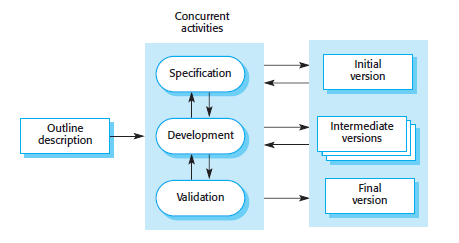
\includegraphics[width=0.70\linewidth]{img/incremental_development.png}
	\caption{Modello di sviluppo incrementale}
\end{figure}

\pagebreak
\subsubsection{Incrementi individuati}
Durante i periodi di Progettazione e Codifica per la Technology Baseline e Progettazione di Dettaglio sono stati individuati alcuni incrementi. \\
Di seguito verranno indicati tutti gli incrementi sviluppati con i relativi requisiti.

\begin{longtable}{C{4cm} L{3cm}}
\rowcolor{white}\caption{Tracciamento incrementi} \\
		\rowcolor{redafk}
\textcolor{white}{\textbf{Incremento}} &
\textcolor{white}{\textbf{Requisiti}} \\
		\endfirsthead
		\rowcolor{white}\caption[]{(continua)} \\
		\rowcolor{redafk}
\textcolor{white}{\textbf{Incremento}} &
\textcolor{white}{\textbf{Requisiti}} \\
		\endhead
Incremento 1: Sviluppo del tool di addestramento e conseguente ottenimento file JSON & Re1F1 \newline Re1F1.1  \newline Re1F1.2 \newline Re1F1.3 \newline Re2F1.6 \newline Re1F1.7 \newline Re1F13 \\
Incremento 2: Caricamento file JSON	nel plug-in & Re1F2 \newline Re1F2.1 \newline Re1F2.2  \newline Re1F2.4\\
Incremento 3: Collegamento plug-in al flusso dati & Re1F3.1 \newline Re1F3.2
\\
Incremento 4: Completamento tool di addestramento & Re1F1.4 \newline Re2F1.5 \newline Re1F11 \newline Re1F12
\\
Incremento 5: Completamento caricamento file JSON nel plugin & Re2F2.3
\\
Incremento 6: Collegamento del predittore al flusso dati e visualizzazione collegamenti & Re1F3.5 \newline Re1F4
\\
Incremento 7: Completamento pannello di collegamento & Re1F3 \newline Re1F3.4
\\
Incremento 8: Scollegamento dei predittori & Re1F5 \newline Re1F5.1 \newline Re1F5.2 \newline Re1F5.3 \newline Re2F5.4 \newline Re1F5.5 
\\
Incremento 9: \newline Modifica dei predittori & Re1F6 \newline Re1F6.1 \newline Re1F6.2 \newline Re1F6.3 \newline Re2F6.4 \newline Re1F6.5
\\
Incremento 10: Monitoraggio delle previsioni & Re1F7 \newline Re1F7.1 \newline Re2F7.2 \newline
\\
Incremento 11: Salvataggio previsioni sul database & Re1F8 \newline  Re1F8.1 \newline Re1F8.2 \newline Re1F8.3 \newline Re2F8.4 \newline Re1F8.5 \newline Re2F8.6
\\
Incremento 12: Visualizzazione dashboard previsioni  & Re1F10 \newline Re1F10.1
\\
Incremento 13: Interruzione monitoraggio & Re1F9 \newline Re1F9.1 \newline Re2F9.2
\\
Incremento 14: Inserimento messaggi di notifica/errori mancanti & Re1F14 \newline Re1F16 \newline Re1F17 \newline Re1F18
\\ 
\end{longtable}
\pagebreak
\subsection{Modello a componenti}
Per la realizzazione del prodotto sarà anche utilizzato, quando possibile, il modello di sviluppo a componenti, così da velocizzare e standardizzare lo
sviluppo dei requisti. I componenti evidenziati dall’analisi sono principalmente
gli elementi esistenti di Grafana e gli algoritmi di predizione (RL e SVM) forniti
da \textit{Zucchetti SPA}. In particolare tali elementi vengono inquadrati nelle seguenti classi di componenti: \begin{itemize}
\item \textbf{Grafana}: sono le librerie e le funzionalità fornite da Grafana, il loro uso viene quindi inquadrato come component reuse;
\item \textbf{Algoritmi di predizione}: sono gli algoritmi che ci sono stati forniti da \textit{Zucchetti SPA} e saranno riutilizzabili come librerie durante lo sviluppo del plug-in. Il loro uso viene quindi inquadrato come object and
function reuse.
\end{itemize}
\pagebreak

\section{Pianificazione}
Sulla base delle cadenza fissate in §1.6, la ripartizione delle attività di progetto avviene tramite:
\begin{itemize}
\item \textbf{Analisi};
\item \textbf{Consolidamento requisiti};
\item \textbf{Progettazione e codifica per la Technology Baseline};
\item \textbf{Progettazione di dettaglio e codifica};
\item \textbf{Validazione e collaudo}.
\end{itemize}  

\subsection{Analisi}
\textit{Periodo: da 2020-03-16 a 2020-04-13} \\
La fase di analisi è suddivisa nel seguente modo:
\begin{itemize}
\item \textbf{Identificazione degli strumenti}: attività rivolta a determinare gli strumenti da utilizzare per le comunicazioni, stesura dei documenti, versionamento, sviluppo e verifica del sistema;
\item \textbf{Norme di Progetto}: sono l'insieme delle regole da seguire per lo svolgimento dei processi e la realizzazione del prodotto. Il documento \textit{Norme di Progetto}, è redatto dall'\textit{Amministratore};
\item \textbf{Studio di Fattibilità}: attività svolta dagli \textit{Analisti} con lo scopo di analizzare i capitolati, in linea generale, per stabilire quale di essi sia una proposta realizzabile. Inoltre è un'attività propedeutica all'\textit{Analisi dei Requisiti};
\item \textbf{Analisi dei Requisiti}: sulla base dell'attività precedente, vengono identificati e definiti i requisiti del sistema. Come per il documento \textit{Studio di Fattibilità}, anche \textit{Analisi dei Requisiti}, viene redatto dagli \textit{Analisti};
\item \textbf{Piano di Qualifica}: attività dell'\textit{Amministratore} e del \textit{Progettista} che si occupa di stabilire le metodologie per garantire la qualità del prodotto. In particolar modo la seconda figura si focalizza sulla parte programmatica;
\item \textbf{Piano di Progetto}: il lavoro da svolgere viene suddiviso in compiti, risorse e attività da parte del \textit{Responsabile}, che ha anche il compito di calcolare il preventivo di periodo del progetto. Il tutto viene riportato sempre da parte del \textit{Responsabile} nel documento \textit{Piano di Progetto};
\item \textbf{Glossario}: tutti i vocaboli di difficile interpretazione vengono individuati riportati nel documento \textit{Glossario}.
\end{itemize}

\begin{figure}[H]
\centering
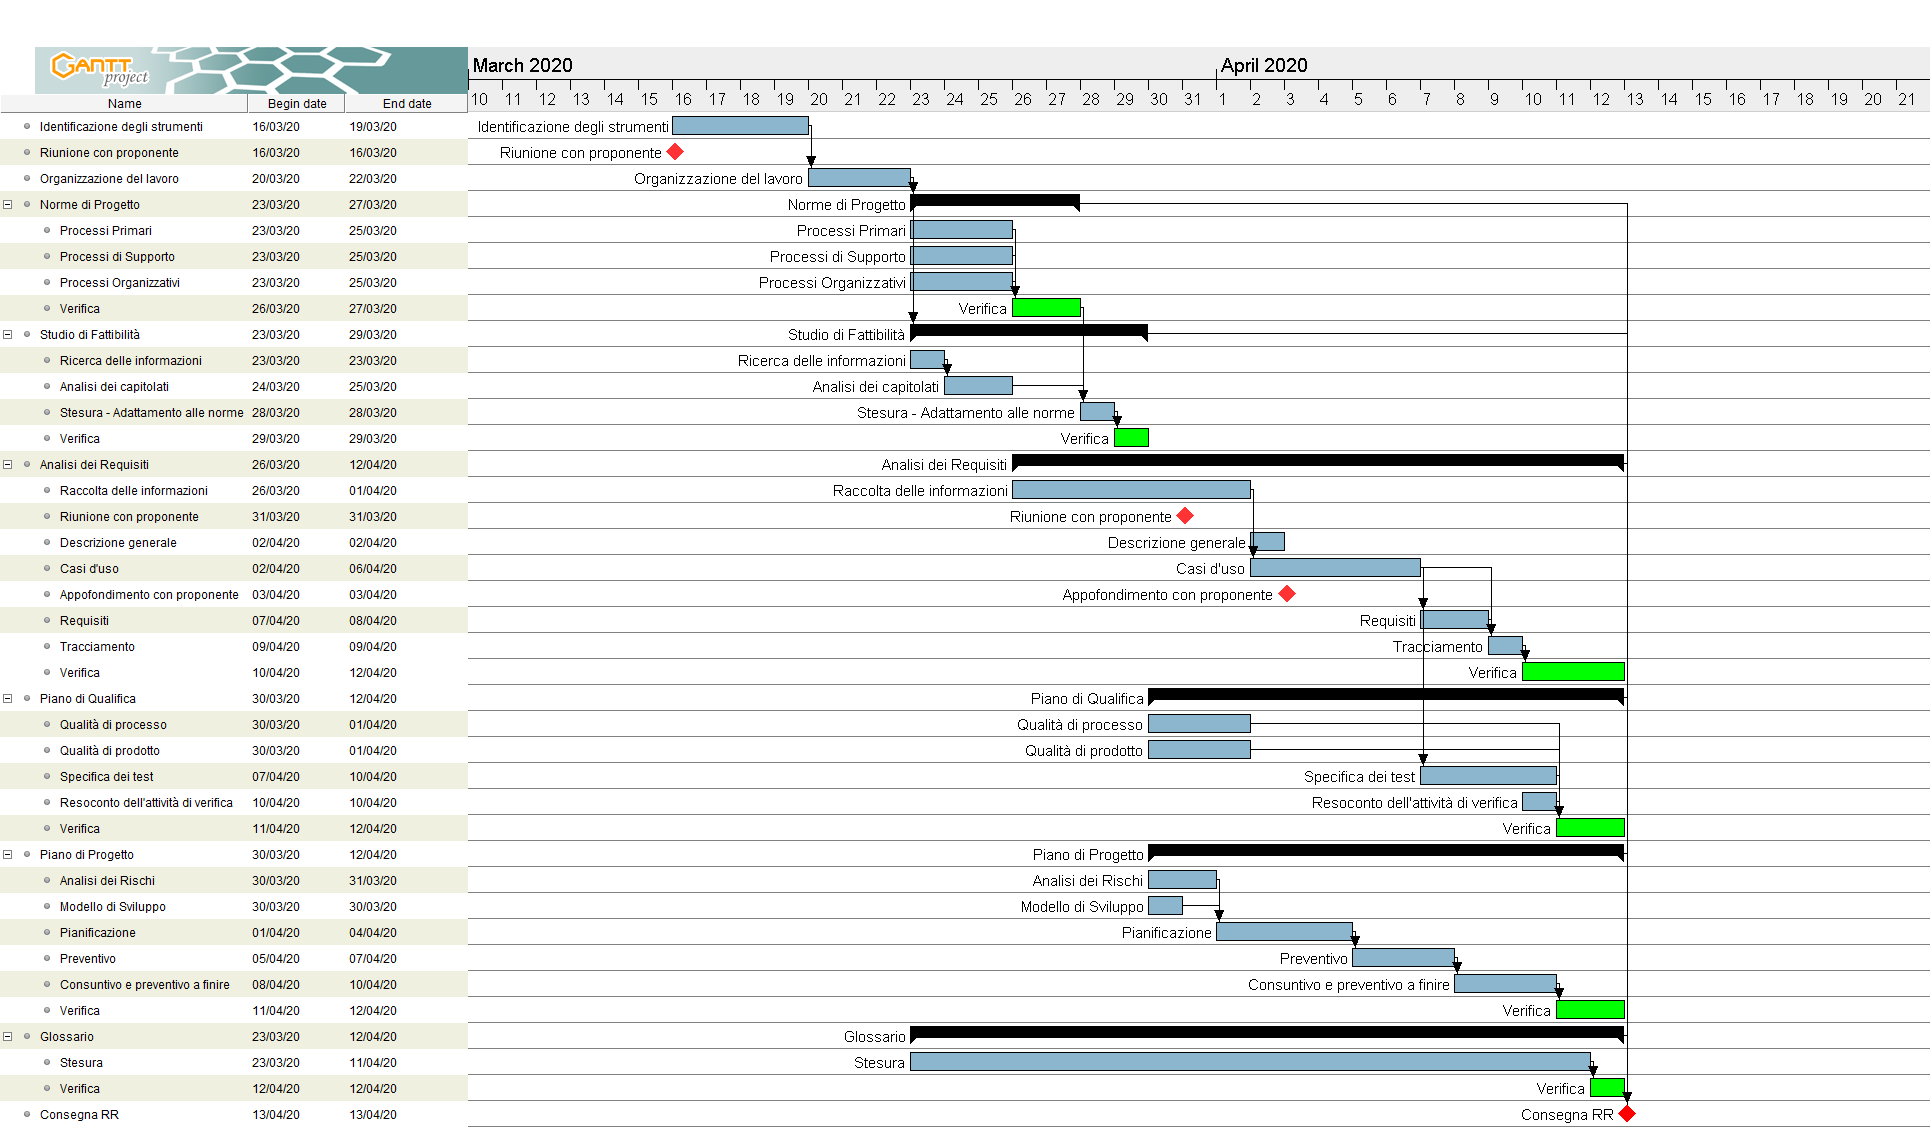
\includegraphics[scale=0.24]{./img/gantt/analisi.png}
\caption{Diagramma di Gantt della fase di Analisi}
\end{figure}

\subsection{Consolidamento dei requisiti}
\textit{Periodo: da 2020-04-14 a 2020-04-20}\\
La fase di consolidamento è così suddivisa:
\begin{itemize}
\item \textbf{Approfondimento personale}: attività intenta a fissare ed approfondire le informazioni riguardanti i requisiti evidenziati nella precedente fase;
\item \textbf{Raccolta informazioni}: raccolta delle informazioni necessarie per la presentazione;
\item \textbf{Stesura presentazione}: preparazione del materiale necessario alla presentazione del 2020-04-20;
\item \textbf{Studio personale}: tempo dedicato ai membri del gruppo, per studiare le informazioni contenute nella presentazione.
\end{itemize}

\begin{figure}[H]
\centering
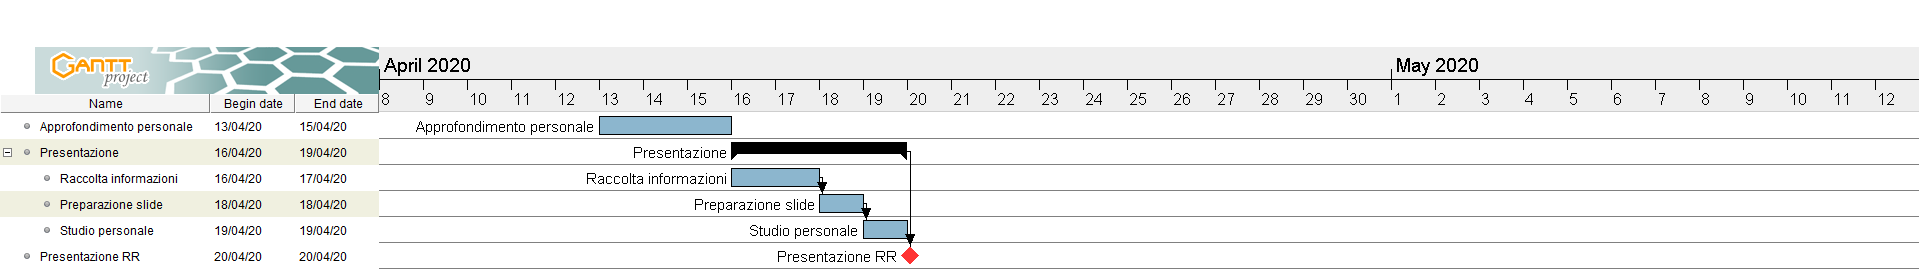
\includegraphics[scale=0.24]{./img/gantt/consolidamento_requisiti.png}
\caption{Diagramma di Gantt della fase di Consolidamento dei requisiti}
\end{figure}

\subsection{Progettazione e codifica per la Technology Baseline}
\textit{Periodo: da 2020-04-21 a 2020-05-11}\\
Questa fase coincide con il giorno successivo alla presentazione del 2020-04-20 e termina con la consegna del materiale per la \textbf{Revisone di Progettazione}. La fase è così suddivisa in:
\begin{itemize}
\item \textbf{Incrementi e verifica}: sulla base dei feedback del committente e del proponente, viene migliorato e verificato il materiale del precedente rilascio.
\item \textbf{Technology Baseline}: vengono identificati i design pattern\glo necessari allo sviluppo del sistema e verranno riportati nell'allegato tecnico insieme al tracciamento dei requisiti. Inoltre viene presentato, al committente e al proponente, un prototipo per mezzo di un repository\glo. In questo periodo saranno implementati solo una parte di requisiti, ovvero quelli che ricoprono le funzionalità di base. Successivamente verranno raffinati i requisiti già implementati, se non completi, e saranno implementate le funzionalità che permetteranno di soddisfare tutti i requisiti. Per fare ciò sono stati individuati i seguenti incrementi:
	\begin{itemize}
		\item \textbf{Incremento 1: ottenimento file JSON:} verrà implementata una pagina web per ottenere il file JSON, mediante l'uso della libreria di React;
		\item \textbf{Incremento 2: caricamento file JSON:} verrà implementata la funzionalità per l'inserimento nel plugin del file JSON, contenente i predittori. Verrà usato React in sinergia con gli strumenti di sviluppo di plugin offerti dalla piattaforma Grafana;
		\item \textbf{Incremento 3: collegamento al flusso dati:} verrà implementata la funzione di collegamento del plugin ad un flusso di dati;
	\end{itemize}
\end{itemize}

\begin{figure}[H]
\centering
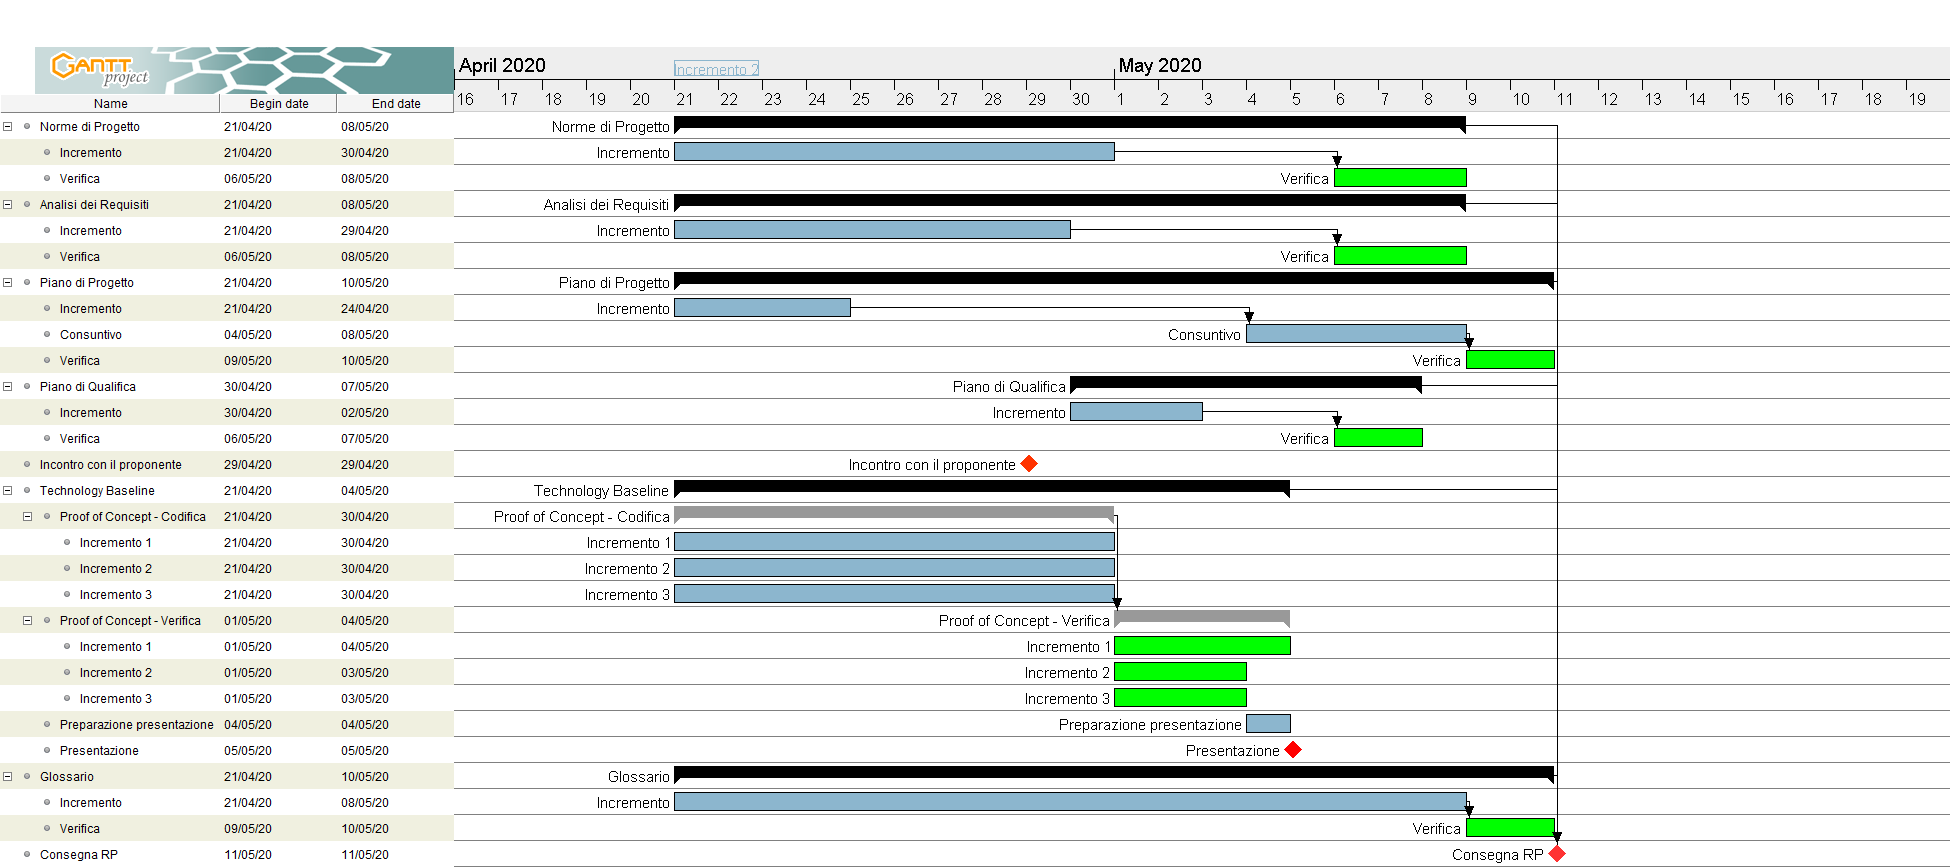
\includegraphics[scale=0.24]{./img/gantt/progettazione_architetturale.png}
\caption{Diagramma di Gantt della fase di Progettazione e codifica per la Technology Baseline}
\end{figure}

\subsection{Progettazine di dettaglio e codifica}
\textit{Periodo: da 2020-05-11 a 2020-06-11}\\
Questa fase è compresa tra il giorno successivo alla presentazione del 2020-05-11 e la consegna della \textit{Revisione di Qualifica}.
\begin{itemize}
\item \textbf{Product Baseline}: le singole unità di cui è composta l'architettura definita nella \textit{Technology Baseline}, vengono ulteriormente analizzate;
\item \textbf{Incrementi e verifica}: sulla base dei feedback del committente e del proponente, viene migliorato e verificato il materiale del precedente rilascio.
\end{itemize}

\begin{figure}[H]
\centering
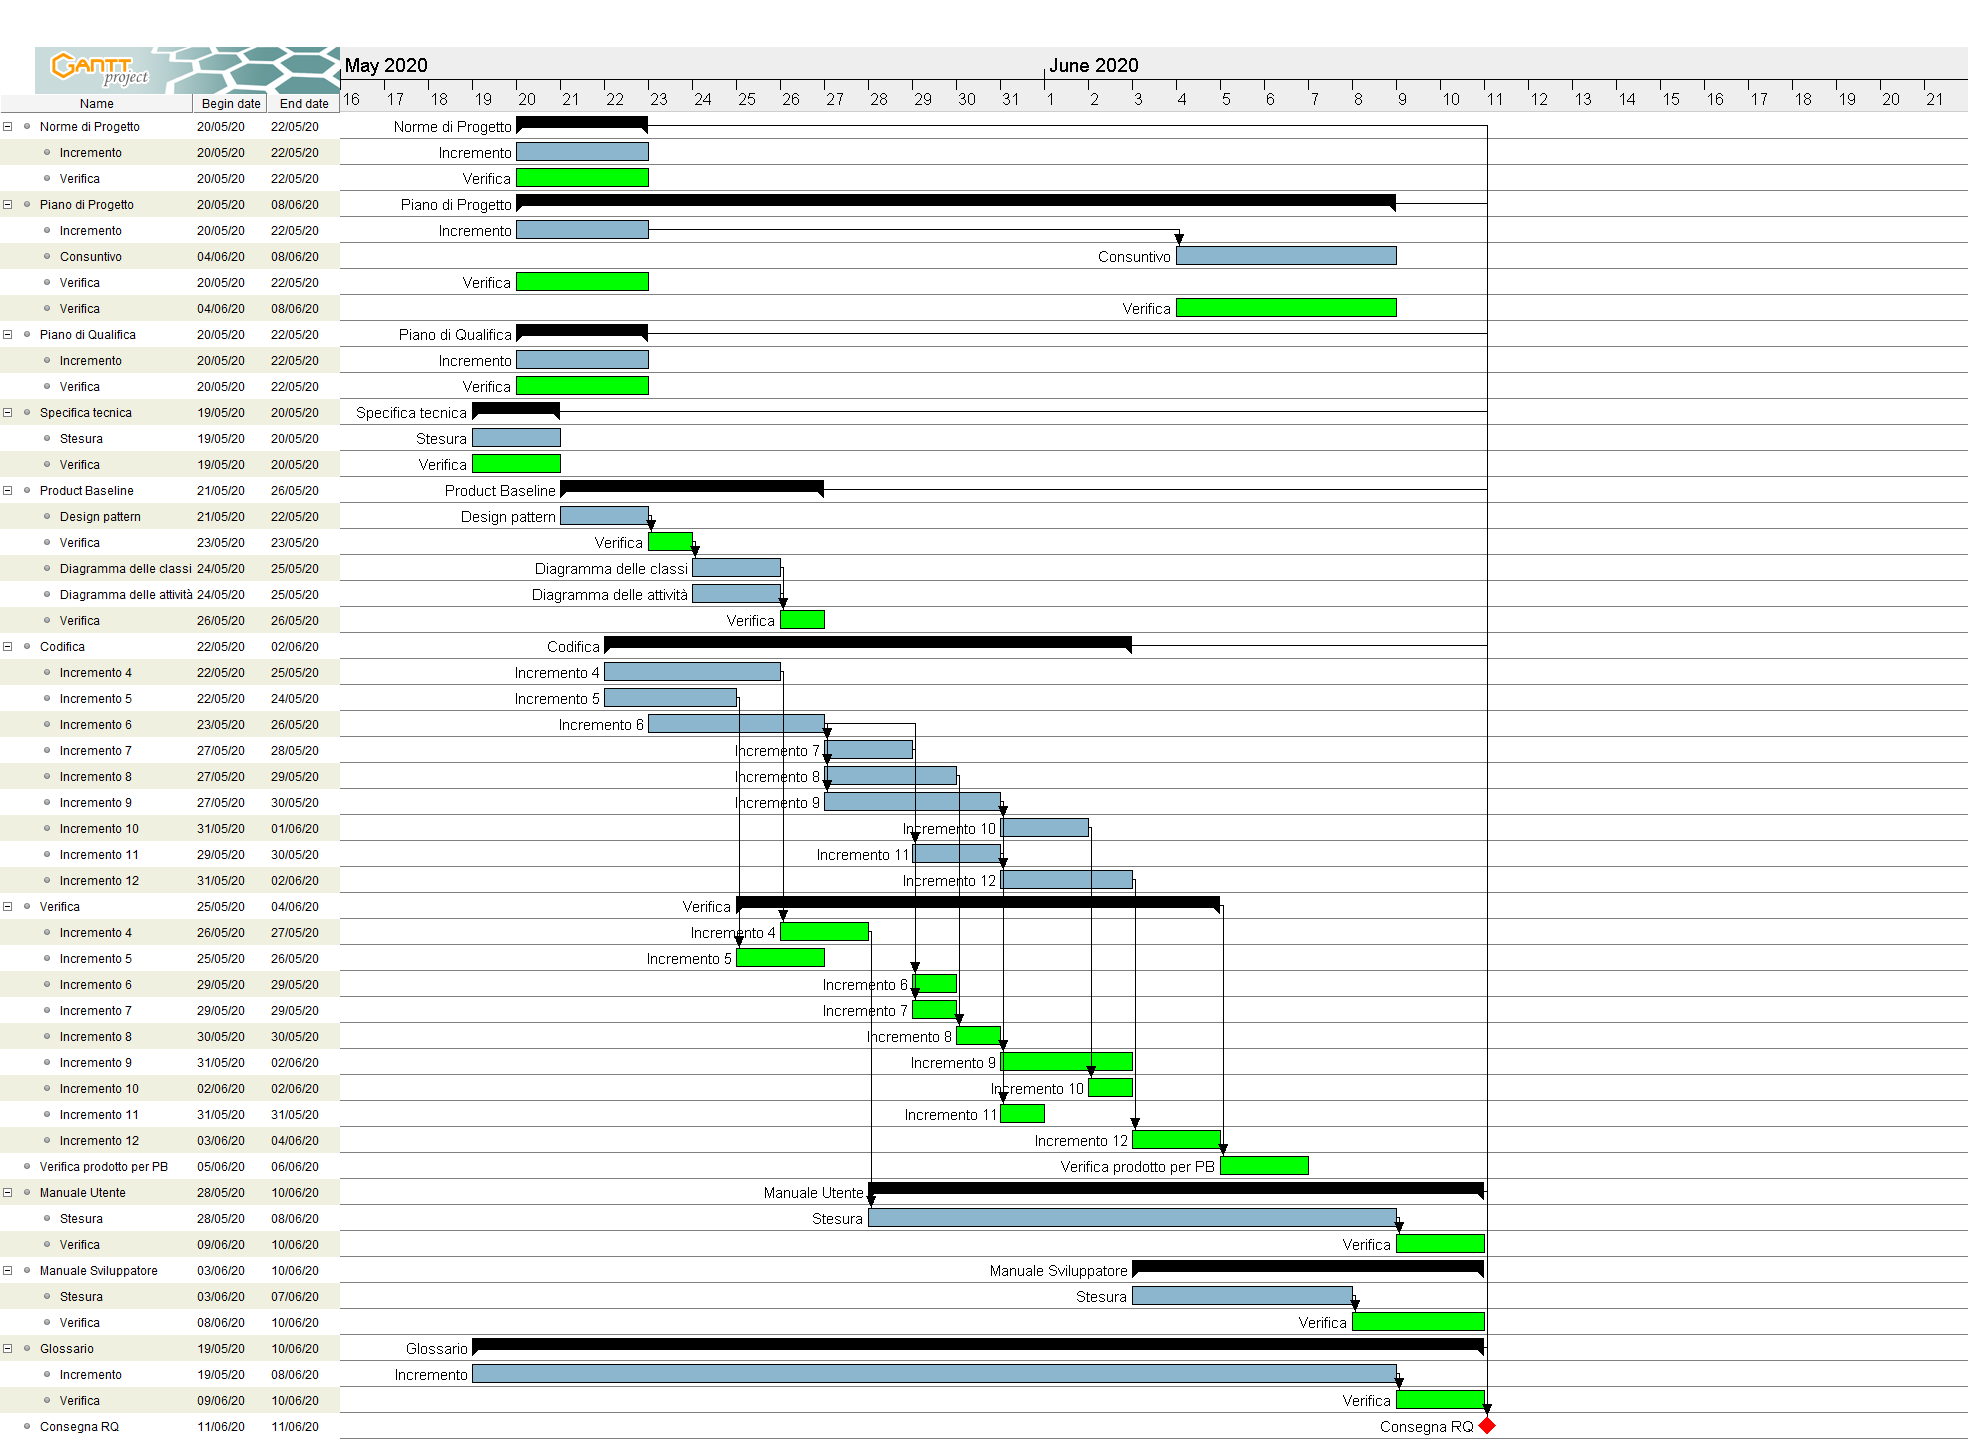
\includegraphics[scale=0.24]{./img/gantt/progettazione_dettaglio_codifica.png}
\caption{Diagramma di Gantt della fase di Progettazione di dettaglio e codifica}
\end{figure}

\subsection{Validazione e collaudo}
\textit{Periodo: da 2020-06-19 a 2020-07-06}\\
La seguente fase inizia il giorno seguente la \textit{Revisione di Qualifica} e termina con la consegna del materiale richiesto per la \textit{Revisione di Avanzamento}.
\begin{itemize}
\item \textbf{Incremento}: nel caso risultasse necessario vengono effettuati miglioramenti sulla base di feedback;
\item \textbf{Validazione e collaudo}: la validazione effettua test sul prodotto, me tre la convalidazione controlla se viene rispettata la coerenza tra il prodotto e le specifiche evidenziate nel documento \textit{Analisi dei Requisiti};
\item \textbf{Manuale Sviluppatore}: viene redatto il documento \textit{Manuale dello Sviluppatore}, il quale conterrà le informazioni necessarie allo sviluppo, mantenimento e manutenzione del prodotto;
\item \textbf{Manuale Utente}: viene redatto il documento \textit{Manuale dell'Utente}, il quale conterrà le informazioni necessarie all'utilizzo del prodotto.
\end{itemize}

\begin{figure}[H]
\centering
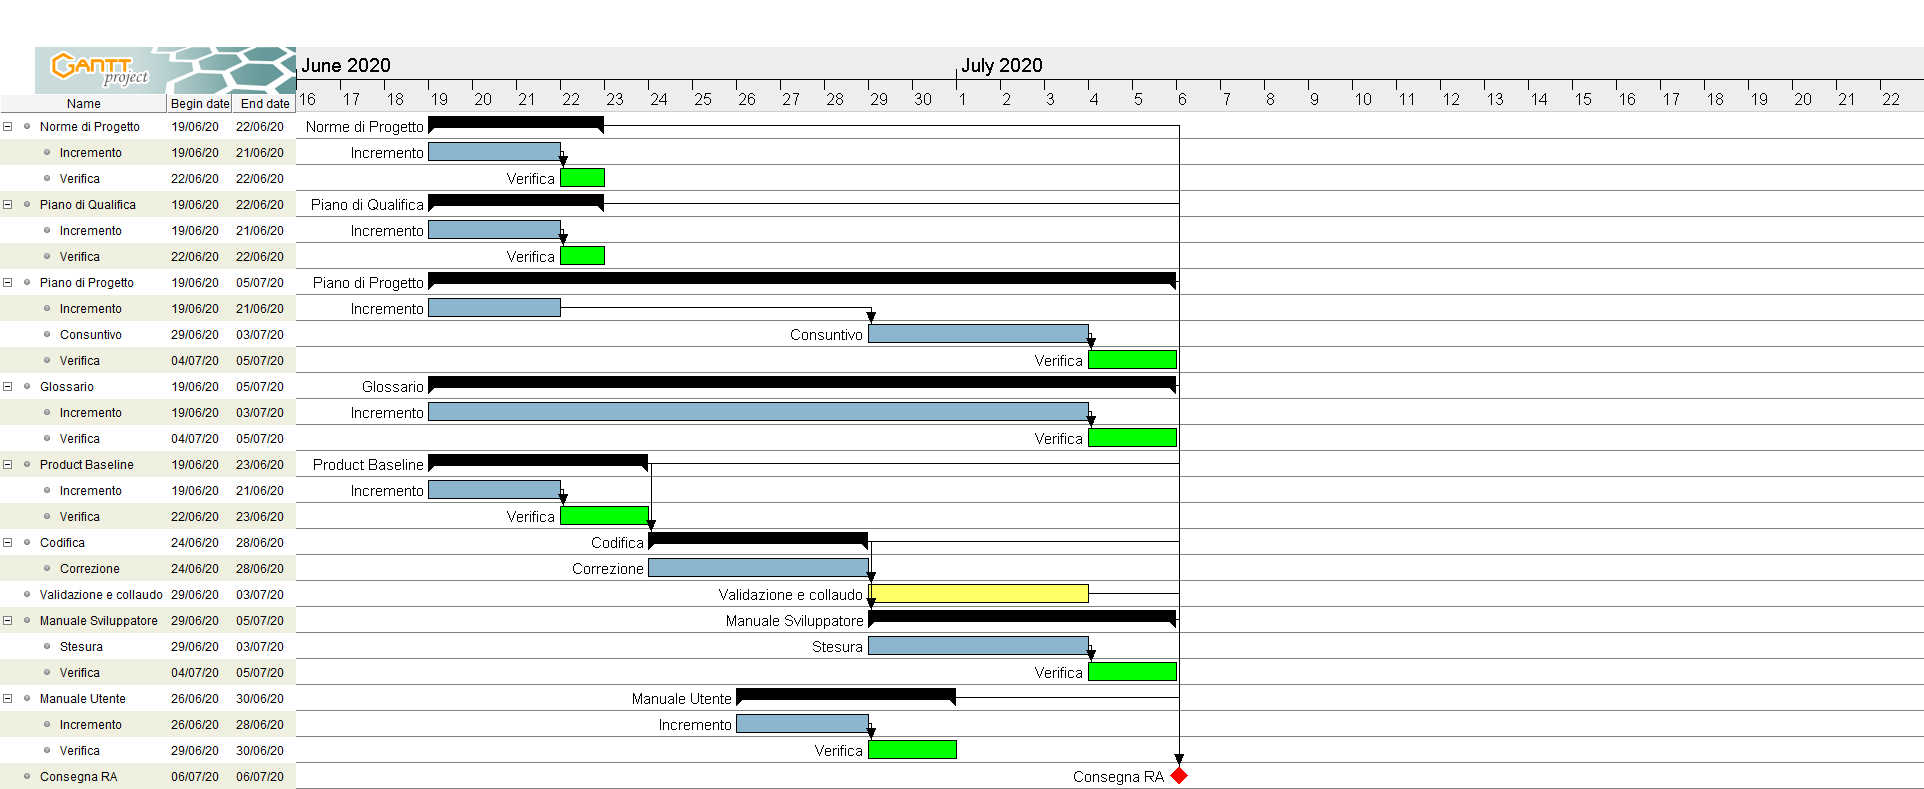
\includegraphics[scale=0.24]{./img/gantt/validazione_collaudo.png}
\caption{Diagramma di Gantt della fase di Validazione e collaudo}
\end{figure}
\pagebreak

\section{Preventivo}
Per facilitare la lettura delle tabelle vengono utilizzate le seguenti sigle per identificare i diversi ruoli e per ognuno di essi vengono indicati i relativi costi/h: \begin{itemize}
\item \textbf{Re}: \textit{Responsabile} 30€/h;
\item \textbf{Am}: \textit{Amministratore} 20€/h;
\item \textbf{An}: \textit{Analista} 25€/h;
\item \textbf{Pt}: \textit{Progettista} 22€/h;
\item \textbf{Pm}: \textit{Programmatore} 15€/h;
\item \textbf{Ve}: \textit{Verificatore} 15€/h.
\end{itemize}
Inoltre, se le ore ricoperte in un determinato ruolo fossero nulle, la cella presenterà il simbolo "-" per indicarne l'assenza.
 
\subsection{Periodo di Analisi}
\subsubsection{Distribuzione oraria}
In questa fase, i ruoli sono così suddivisi:
\begin{table}[H]
\centering\renewcommand{\arraystretch}{1.5}
\caption{Distribuzione delle ore nella fase di Analisi}
\vspace{0.2cm}
\begin{tabular}{ c c c c c c c c }
\rowcolor{redafk}
\textcolor{white}{\textbf{Nominativo}} & \textcolor{white}{\textbf{Re}} &
\textcolor{white}{\textbf{Am}} & \textcolor{white}{\textbf{An}} &
\textcolor{white}{\textbf{Pt}} & \textcolor{white}{\textbf{Pm}} &
\textcolor{white}{\textbf{Ve}} & \textcolor{white}{\textbf{Totale}} \\
Simone Federico Bergamin & 6 & 7 & 20 & - & - & 9 & 42 \\
Alessandro Canesso & 8 & 6 & 16 & - & - & 12 & 42 \\
Victor Dutca & 9 & - & 15 & - & - & 16 & 40 \\
Fouad Farid & 7 & 7 & 12 & 6 & - & 8 & 40 \\
Simone Meneghin & - & 8 & 14 & 10 & - & 10 & 42 \\
Olivier Utshudi & - & 8 & 13 & 8 & - & 13 & 42 \\
Davide Zilio & 4 & 5 & 17 & - & - & 14 & 40 \\
\rowcolor{lastrowcolor}
\textbf{Ore totali ruolo} & \textbf{34} & \textbf{41} & \textbf{107} & \textbf{24} & \textbf{0} & \textbf{82} & \textbf{288} \\
\end{tabular}
\end{table}
 
\pagebreak
 
I dati ottenuti sono riassunti nel seguente istogramma:
\begin{figure}[H]
\centering
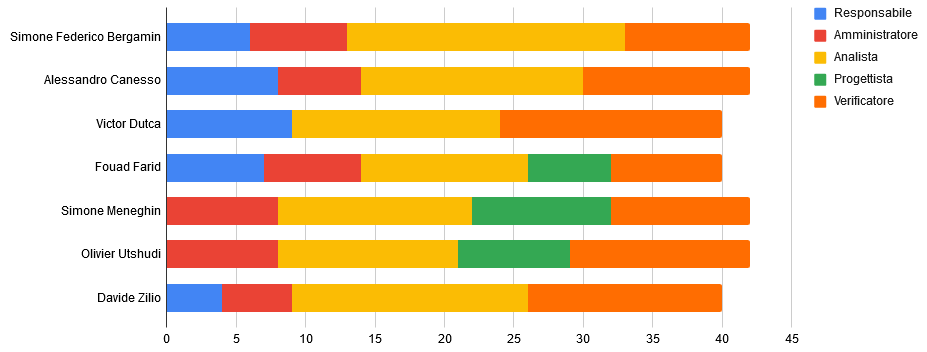
\includegraphics[scale=0.60]{img/grafici/tabella_fase_analisi.png}
\caption{Istogramma della ripartizione delle ore per ruolo nella fase di Analisi}
\end{figure}
 
\subsubsection{Prospetto economico}
In questa fase il costo per ogni ruolo è il seguente:
 
%tabella costi
\begin{table}[H]
\centering\renewcommand{\arraystretch}{1.5}
\caption{Prospetto dei costi nella fase di Analisi}
\vspace{0.2cm}
\begin{tabular}{ c c c  }
\rowcolor{redafk}
\textcolor{white}{\textbf{Ruolo}} & \textcolor{white}{\textbf{Ore}} &
\textcolor{white}{\textbf{Costo}}  \\
Responsabile & 34 & 1020€ \\
Amministratore & 41 & 820€ \\
Analista & 107 & 2675€ \\
Progettista & 24 & 528€ \\
Programmatore & 0 & 0€  \\
Verificatore & 82 & 1230€  \\
\rowcolor{lastrowcolor}
\textbf{Totale} & \textbf{288} & \textbf{6273€}  \\
\end{tabular}
\end{table}
 
I dati ottenuti sono riassunti nel seguente areogramma:
\begin{figure}[H]
\centering
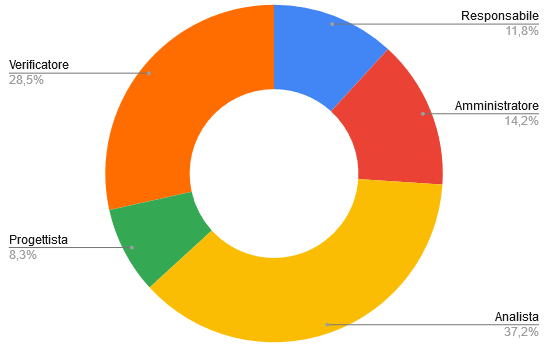
\includegraphics[scale=0.60]{img/grafici/torta_fase_analisi_prospetto_economico.png}
\caption{Areogramma della ripartizione dei costi per ruolo nella fase di Analisi}
\end{figure}
 
%--------------------------------------------------
 
\subsection{Periodo di Progettazione e codifica per la Technology Baseline}
\subsubsection{Distribuzione oraria}
In questa fase i ruoli sono così suddivisi:
\begin{table}[H]
\centering\renewcommand{\arraystretch}{1.5}
\caption{Distribuzione delle ore nella fase di Progettazione e codifica per la Technology Baseline}
\vspace{0.2cm}
\begin{tabular}{ c c c c c c c c }
\rowcolor{redafk}
\textcolor{white}{\textbf{Nominativo}} & \textcolor{white}{\textbf{Re}} &
\textcolor{white}{\textbf{Am}} & \textcolor{white}{\textbf{An}} &
\textcolor{white}{\textbf{Pt}} & \textcolor{white}{\textbf{Pm}} &
\textcolor{white}{\textbf{Ve}} & \textcolor{white}{\textbf{Totale}} \\
Simone Federico Bergamin & - & - & 10 & 7 & 5 & 8 & 30 \\
Alessandro Canesso & - & 5 & - & 10 & 9 & 8 & 32 \\
Victor Dutca & 3 & 6 & 4 & 10 & 7 & - & 30 \\
Fouad Farid & - & 5 & - & 14 & - & 11 & 30 \\
Simone Meneghin & 6 & - & 8 & 10 & 6 & - & 30 \\
Olivier Utshudi & - & 4 & - & 8 & 6 & 12 & 30 \\
Davide Zilio & 3 & - & 13 & - & - & 14 & 30 \\
\rowcolor{lastrowcolor}
\textbf{Ore totali ruolo} & \textbf{12} & \textbf{20} & \textbf{35} & \textbf{59} & \textbf{33} & \textbf{53} & \textbf{212} \\
\end{tabular}
\end{table}
 
I dati ottenuti sono riassunti nel seguente istogramma:
\begin{figure}[H]
\centering
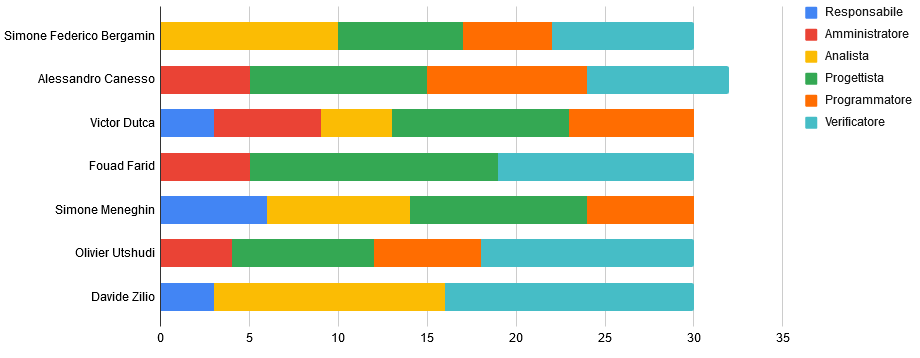
\includegraphics[scale=0.60]{img/grafici/tabella_fase_prog_architetturale.png}
\caption{Istogramma della ripartizione delle ore per ruolo nella fase di Progettazione e codifica per la Technology Baseline}
\end{figure}
 
\subsubsection{Prospetto economico}
In questa fase il costo per ogni ruolo è il seguente:
 
%tabella costi
\begin{table}[H]
\centering\renewcommand{\arraystretch}{1.5}
\caption{Prospetto dei costi nella fase di Progettazione e codifica per la Technology Baseline}
\vspace{0.2cm}
\begin{tabular}{ c c c }
\rowcolor{redafk}
\textcolor{white}{\textbf{Ruolo}} & \textcolor{white}{\textbf{Ore}} &
\textcolor{white}{\textbf{Costo}}  \\
Responsabile & 12 & 360€ \\
Amministratore & 20 & 400€ \\
Analista & 35 & 875€ \\
Progettista & 59 & 1298€ \\
Programmatore & 33 & 495€  \\
Verificatore & 53 & 795€  \\
\rowcolor{lastrowcolor}
\textbf{Totale} & \textbf{212} & \textbf{4223€}  \\
\end{tabular}
\end{table}
 
I dati ottenuti sono riassunti nel seguente areogramma:
\begin{figure}[H]
\centering
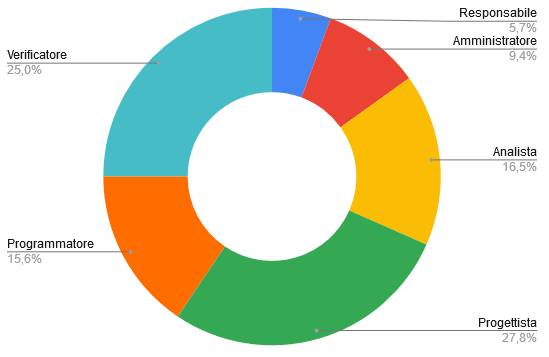
\includegraphics[scale=0.60]{img/grafici/torta_fase_prog_architetturale.png}
\caption{Areogramma della ripartizione dei costi per ruolo nella fase di Progettazione e codifica per la Technology Baseline}
\end{figure}
 
%--------------------------------------------------
 
\subsection{Periodo di Progettazione di dettaglio e codifica}
\subsubsection{Distribuzione oraria}
In questa fase i ruoli sono così suddivisi:
\begin{table}[H]
\centering\renewcommand{\arraystretch}{1.5}
\caption{Distribuzione delle ore nella fase di Progettazione di dettaglio e codifica}
\vspace{0.2cm}
\begin{tabular}{ c c c c c c c c }
\rowcolor{redafk}
\textcolor{white}{\textbf{Nominativo}} & \textcolor{white}{\textbf{Re}} &
\textcolor{white}{\textbf{Am}} & \textcolor{white}{\textbf{An}} &
\textcolor{white}{\textbf{Pt}} & \textcolor{white}{\textbf{Pm}} &
\textcolor{white}{\textbf{Ve}} & \textcolor{white}{\textbf{Totale}} \\
Simone Federico Bergamin & - & 6 & - & 12 & 18 & 12 & 48 \\
Alessandro Canesso & 4 & 3 & - & 10 & 18 & 11 & 46 \\
Victor Dutca & - & 8 & - & 10 & 20 & 10 & 48 \\
Fouad Farid & 4 & - & - & 12 & 20 & 12 & 48 \\
Simone Meneghin & 2 & - & - & 12 & 22 & 14 & 50 \\
Olivier Utshudi & 8 & - & - & 8 & 22 & 12 & 50 \\
Davide Zilio & - & 6 & - & 10 & 20 & 12 & 48 \\
\rowcolor{lastrowcolor}
\textbf{Ore totali ruolo} & \textbf{18} & \textbf{23} & \textbf{0} & \textbf{74} & \textbf{140} & \textbf{83} & \textbf{338} \\
\end{tabular}
\end{table}
 
I dati ottenuti sono riassunti nel seguente istogramma:
\begin{figure}[H]
\centering
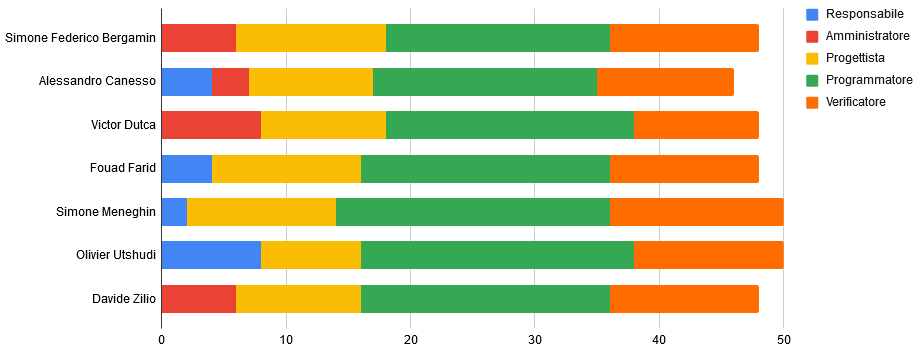
\includegraphics[scale=0.60]{img/grafici/tabella_fase_prog_cod.png}
\caption{Istogramma della ripartizione delle ore per ruolo nella fase di Progettazione di dettaglio e codifica}
\end{figure}

\paragraph{Distribuzione oraria incrementi}
\paragraph*{Incremento 4} \mbox{} \\
\begin{table}[H]
\centering\renewcommand{\arraystretch}{1.5}
\caption{Distribuzione delle ore per lo sviluppo dell'incremento 4}
\vspace{0.2cm}
\begin{tabular}{ c c c c c c c c }
\rowcolor{redafk}
\textcolor{white}{\textbf{Nominativo}} & \textcolor{white}{\textbf{Re}} &
\textcolor{white}{\textbf{Am}} & \textcolor{white}{\textbf{An}} &
\textcolor{white}{\textbf{Pt}} & \textcolor{white}{\textbf{Pm}} &
\textcolor{white}{\textbf{Ve}} & \textcolor{white}{\textbf{Totale}} \\
Simone Federico Bergamin & - & - & - & - & - & - & 0 \\
Alessandro Canesso & - & - & - & - & - & - & 0\\
Victor Dutca & - & 2 & - & - & 5 & - & 7 \\
Fouad Farid & - & - & - & - & 11 & - & 11 \\
Simone Meneghin & 2 & - & - & - & - & 6 & 8 \\
Olivier Utshudi & - & - & - & - & - & - & 0 \\
Davide Zilio & - & 2 & - & 4 & - & - & 6 \\
\rowcolor{lastrowcolor}
\textbf{Ore totali ruolo} & \textbf{2} & \textbf{4} & \textbf{0} & \textbf{4} & \textbf{16} & \textbf{6} & \textbf{32} \\
\end{tabular}
\end{table}

I dati ottenuti sono riassunti nel seguente istogramma:
\begin{figure}[H]
\centering
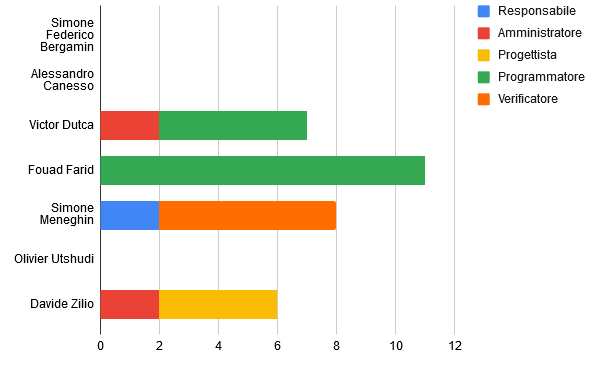
\includegraphics[scale=0.60]{img/grafici/tabella_inc4.png}
\caption{Istogramma della ripartizione delle ore per lo sviluppo dell'incremento 4}
\end{figure}

\paragraph*{Incremento 5}\mbox{} \\
\begin{table}[H]
\centering\renewcommand{\arraystretch}{1.5}
\caption{Distribuzione delle ore per lo sviluppo dell'incremento 5}
\vspace{0.2cm}
\begin{tabular}{ c c c c c c c c }
\rowcolor{redafk}
\textcolor{white}{\textbf{Nominativo}} & \textcolor{white}{\textbf{Re}} &
\textcolor{white}{\textbf{Am}} & \textcolor{white}{\textbf{An}} &
\textcolor{white}{\textbf{Pt}} & \textcolor{white}{\textbf{Pm}} &
\textcolor{white}{\textbf{Ve}} & \textcolor{white}{\textbf{Totale}} \\
Simone Federico Bergamin & - & - & - & - & - & - & 0 \\
Alessandro Canesso & 1 & - & - & 1 & - & 2 & 4 \\
Victor Dutca & - & 1 & - & - & - & - & 1 \\
Fouad Farid & - & - & - & - & - & - & 0 \\
Simone Meneghin & - & - & - & - & - & - & 0 \\
Olivier Utshudi & - & - & - & - & 3 & - & 3 \\
Davide Zilio & - & - & - & - & - & - & 0 \\
\rowcolor{lastrowcolor}
\textbf{Ore totali ruolo} & \textbf{1} & \textbf{1} & \textbf{0} & \textbf{1} & \textbf{3} & \textbf{2} & \textbf{8} \\
\end{tabular}
\end{table}

I dati ottenuti sono riassunti nel seguente istogramma:
\begin{figure}[H]
\centering
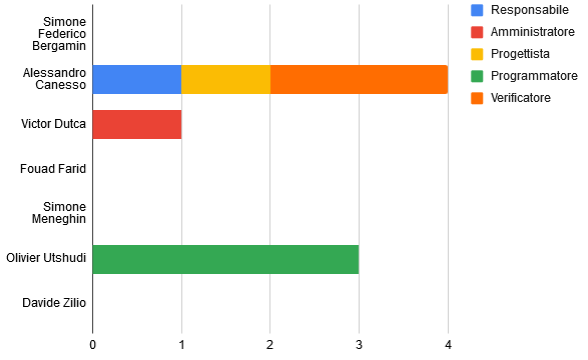
\includegraphics[scale=0.60]{img/grafici/tabella_inc5.png}
\caption{Istogramma della ripartizione delle ore per lo sviluppo dell'incremento 5}
\end{figure}

\paragraph*{Incremento 6}\mbox{} \\
\begin{table}[H]
\centering\renewcommand{\arraystretch}{1.5}
\caption{Distribuzione delle ore per lo sviluppo dell'incremento 6}
\vspace{0.2cm}
\begin{tabular}{ c c c c c c c c }
\rowcolor{redafk}
\textcolor{white}{\textbf{Nominativo}} & \textcolor{white}{\textbf{Re}} &
\textcolor{white}{\textbf{Am}} & \textcolor{white}{\textbf{An}} &
\textcolor{white}{\textbf{Pt}} & \textcolor{white}{\textbf{Pm}} &
\textcolor{white}{\textbf{Ve}} & \textcolor{white}{\textbf{Totale}} \\
Simone Federico Bergamin & - & 2 & - & - & 8 & - & 10 \\
Alessandro Canesso & - & - & - & - & - & 6 & 6 \\
Victor Dutca & - & 2 & - & 2 & - & - & 4 \\
Fouad Farid & - & - & - & 4 & - & - & 4 \\
Simone Meneghin & - & - & - & - & - & - & 0 \\
Olivier Utshudi & 3 & - & - & - & - & - & 3 \\
Davide Zilio & - & - & - & - & 7 & - & 7 \\
\rowcolor{lastrowcolor}
\textbf{Ore totali ruolo} & \textbf{3} & \textbf{4} & \textbf{-} & \textbf{6} & \textbf{15} & \textbf{6} & \textbf{34} \\
\end{tabular}
\end{table}

I dati ottenuti sono riassunti nel seguente istogramma:
\begin{figure}[H]
\centering
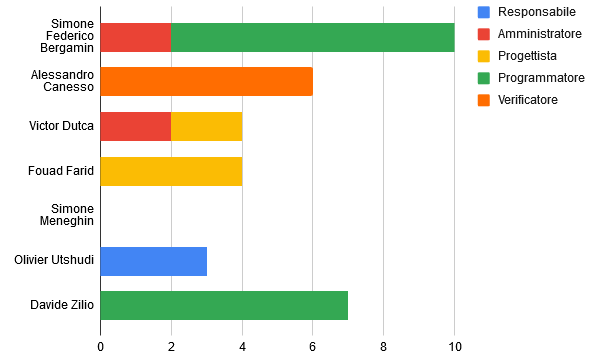
\includegraphics[scale=0.60]{img/grafici/tabella_inc6.png}
\caption{Istogramma della ripartizione delle ore per lo sviluppo dell'incremento 6}
\end{figure}

\paragraph*{Incremento 7}\mbox{} \\
\begin{table}[H]
\centering\renewcommand{\arraystretch}{1.5}
\caption{Distribuzione delle ore per lo sviluppo dell'incremento 7}
\vspace{0.2cm}
\begin{tabular}{ c c c c c c c c }
\rowcolor{redafk}
\textcolor{white}{\textbf{Nominativo}} & \textcolor{white}{\textbf{Re}} &
\textcolor{white}{\textbf{Am}} & \textcolor{white}{\textbf{An}} &
\textcolor{white}{\textbf{Pt}} & \textcolor{white}{\textbf{Pm}} &
\textcolor{white}{\textbf{Ve}} & \textcolor{white}{\textbf{Totale}} \\
Simone Federico Bergamin & - & 2 & - & - & - & - & 2 \\
Alessandro Canesso & 2 & - & - & - & - & - & 2 \\
Victor Dutca & - & - & - & - & - & - & 0 \\
Fouad Farid & - & - & - & - & - & - & 0 \\
Simone Meneghin & - & - & - & 6 & - & - & 6 \\
Olivier Utshudi & - & - & - & 4 & 6 & 4 & 8 \\
Davide Zilio & - & - & - & - & - & - & 0 \\
\rowcolor{lastrowcolor}
\textbf{Ore totali ruolo} & \textbf{2} & \textbf{2} & \textbf{0} & \textbf{10} & \textbf{6} & \textbf{4} & \textbf{24} \\
\end{tabular}
\end{table}

I dati ottenuti sono riassunti nel seguente istogramma:
\begin{figure}[H]
\centering
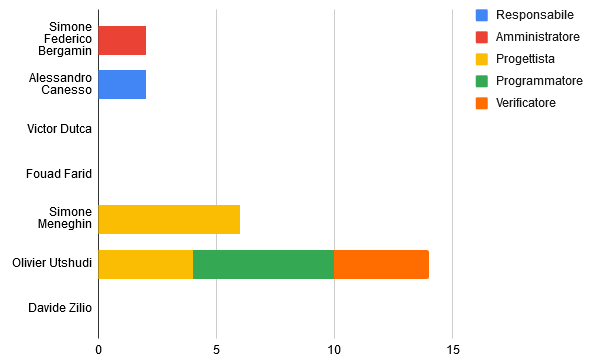
\includegraphics[scale=0.60]{img/grafici/tabella_inc7.png}
\caption{Istogramma della ripartizione delle ore per lo sviluppo dell'incremento 7}
\end{figure}

\paragraph*{Incremento 8}\mbox{} \\
\begin{table}[H]
\centering\renewcommand{\arraystretch}{1.5}
\caption{Distribuzione delle ore per lo sviluppo dell'incremento 8}
\vspace{0.2cm}
\begin{tabular}{ c c c c c c c c }
\rowcolor{redafk}
\textcolor{white}{\textbf{Nominativo}} & \textcolor{white}{\textbf{Re}} &
\textcolor{white}{\textbf{Am}} & \textcolor{white}{\textbf{An}} &
\textcolor{white}{\textbf{Pt}} & \textcolor{white}{\textbf{Pm}} &
\textcolor{white}{\textbf{Ve}} & \textcolor{white}{\textbf{Totale}} \\
Simone Federico Bergamin & - & - & - & 4 & - & - & 4 \\
Alessandro Canesso & - & - & - & - & 6 & - & 6 \\
Victor Dutca & - & - & - & - & - & 6 & 6 \\
Fouad Farid & - & - & - & - & - & 5 & 5 \\
Simone Meneghin & - & - & - & - & 8 & - & 8 \\
Olivier Utshudi & 3 & - & - & 4 & - & - & 7 \\
Davide Zilio & - & 4 & - & - & 6 & - & 10 \\
\rowcolor{lastrowcolor}
\textbf{Ore totali ruolo} & \textbf{3} & \textbf{4} & \textbf{0} & \textbf{8} & \textbf{20} & \textbf{11} & \textbf{46} \\
\end{tabular}
\end{table}

I dati ottenuti sono riassunti nel seguente istogramma:
\begin{figure}[H]
\centering
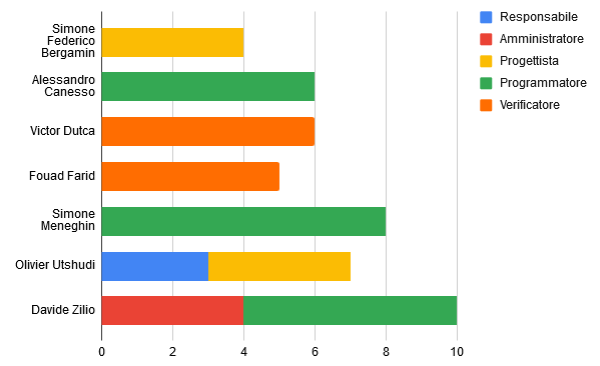
\includegraphics[scale=0.60]{img/grafici/tabella_inc8.png}
\caption{Istogramma della ripartizione delle ore per lo sviluppo dell'incremento 8}
\end{figure}

\paragraph*{Incremento 9}\mbox{} \\
\begin{table}[H]
\centering\renewcommand{\arraystretch}{1.5}
\caption{Distribuzione delle ore per lo sviluppo dell'incremento 9}
\vspace{0.2cm}
\begin{tabular}{ c c c c c c c c }
\rowcolor{redafk}
\textcolor{white}{\textbf{Nominativo}} & \textcolor{white}{\textbf{Re}} &
\textcolor{white}{\textbf{Am}} & \textcolor{white}{\textbf{An}} &
\textcolor{white}{\textbf{Pt}} & \textcolor{white}{\textbf{Pm}} &
\textcolor{white}{\textbf{Ve}} & \textcolor{white}{\textbf{Totale}} \\
Simone Federico Bergamin & - & 2 & - & 4 & 8 & - & 14\\
Alessandro Canesso & - & 2 & - & 5 & - & - & 7 \\
Victor Dutca & - & - & - & - & 10 & - & 10 \\
Fouad Farid & - & - & - & - & 9 & - & 9 \\
Simone Meneghin & - & - & - & - & - & 8 & 8 \\
Olivier Utshudi & 2 & - & - & - & - & 8 & 10 \\
Davide Zilio & - & - & - & 6 & - & 4 & 10 \\
\rowcolor{lastrowcolor}
\textbf{Ore totali ruolo} & \textbf{2} & \textbf{4} & \textbf{0} & \textbf{15} & \textbf{27} & \textbf{20} & \textbf{68} \\
\end{tabular}
\end{table}

I dati ottenuti sono riassunti nel seguente istogramma:
\begin{figure}[H]
\centering
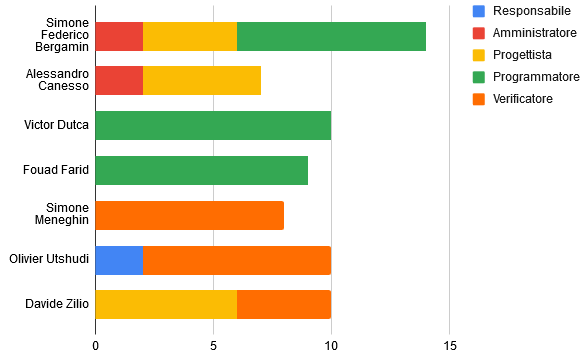
\includegraphics[scale=0.60]{img/grafici/tabella_inc9.png}
\caption{Istogramma della ripartizione delle ore per lo sviluppo dell'incremento 9}
\end{figure}

\paragraph*{Incremento 10}\mbox{} \\
\begin{table}[H]
\centering\renewcommand{\arraystretch}{1.5}
\caption{Distribuzione delle ore per lo sviluppo dell'incremento 10}
\vspace{0.2cm}
\begin{tabular}{ c c c c c c c c }
\rowcolor{redafk}
\textcolor{white}{\textbf{Nominativo}} & \textcolor{white}{\textbf{Re}} &
\textcolor{white}{\textbf{Am}} & \textcolor{white}{\textbf{An}} &
\textcolor{white}{\textbf{Pt}} & \textcolor{white}{\textbf{Pm}} &
\textcolor{white}{\textbf{Ve}} & \textcolor{white}{\textbf{Totale}} \\
Simone Federico Bergamin & - & - & - & - & 2 & 5 & 7 \\
Alessandro Canesso & 1 & 1 & - & 4 & - & - & 6 \\
Victor Dutca & - & - & - & - & 5 & 4 & 9 \\
Fouad Farid & - & - & - & 3 & - & - & 3  \\
Simone Meneghin & - & - & - & - & 4 & - & 4 \\
Olivier Utshudi & - & - & - & - & - & - & 0 \\
Davide Zilio & - & - & - & - & - & - & 0 \\
\rowcolor{lastrowcolor}
\textbf{Ore totali ruolo} & \textbf{1} & \textbf{1} & \textbf{0} & \textbf{7} & \textbf{11} & \textbf{9} & \textbf{29} \\
\end{tabular}
\end{table}

I dati ottenuti sono riassunti nel seguente istogramma:
\begin{figure}[H]
\centering
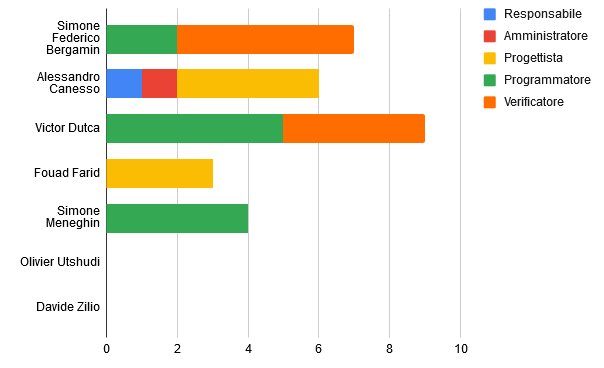
\includegraphics[scale=0.60]{img/grafici/tabella_inc10.png}
\caption{Istogramma della ripartizione delle ore per lo sviluppo dell'incremento 10}
\end{figure}

\paragraph*{Incremento 11}\mbox{} \\
\begin{table}[H]
\centering\renewcommand{\arraystretch}{1.5}
\caption{Distribuzione delle ore per lo sviluppo dell'incremento 11}
\vspace{0.2cm}
\begin{tabular}{ c c c c c c c c }
\rowcolor{redafk}
\textcolor{white}{\textbf{Nominativo}} & \textcolor{white}{\textbf{Re}} &
\textcolor{white}{\textbf{Am}} & \textcolor{white}{\textbf{An}} &
\textcolor{white}{\textbf{Pt}} & \textcolor{white}{\textbf{Pm}} &
\textcolor{white}{\textbf{Ve}} & \textcolor{white}{\textbf{Totale}} \\
Simone Federico Bergamin & - & - & - & - & - & 3 & 3\\
Alessandro Canesso & - & - & - & - & 6 & - & 6 \\
Victor Dutca & - & 3 & - & 5 & - & - & 8 \\
Fouad Farid & 2 & - & - & - & - & 7 & 9 \\
Simone Meneghin & - & - & - & 6 & - & - & 6 \\
Olivier Utshudi & - & - & - & - & 5 & - & 5 \\
Davide Zilio & - & - & - & - & 7 & - & 7 \\
\rowcolor{lastrowcolor}
\textbf{Ore totali ruolo} & \textbf{2} & \textbf{3} & \textbf{0} & \textbf{11} & \textbf{18} & \textbf{10} & \textbf{44} \\
\end{tabular}
\end{table}

I dati ottenuti sono riassunti nel seguente istogramma:
\begin{figure}[H]
\centering
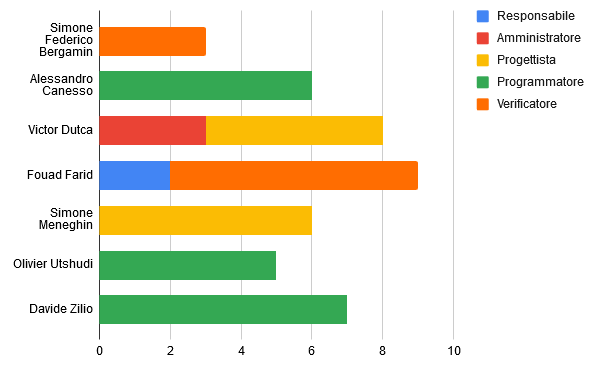
\includegraphics[scale=0.60]{img/grafici/tabella_inc11.png}
\caption{Istogramma della ripartizione delle ore per lo sviluppo dell'incremento 11}
\end{figure}

\paragraph*{Incremento 12}\mbox{} \\
\begin{table}[H]
\centering\renewcommand{\arraystretch}{1.5}
\caption{Distribuzione delle ore per lo sviluppo dell'incremento 12}
\vspace{0.2cm}
\begin{tabular}{ c c c c c c c c }
\rowcolor{redafk}
\textcolor{white}{\textbf{Nominativo}} & \textcolor{white}{\textbf{Re}} &
\textcolor{white}{\textbf{Am}} & \textcolor{white}{\textbf{An}} &
\textcolor{white}{\textbf{Pt}} & \textcolor{white}{\textbf{Pm}} &
\textcolor{white}{\textbf{Ve}} & \textcolor{white}{\textbf{Totale}} \\
Simone Federico Bergamin & - & - & - & 4 & - & 4 & 8 \\
Alessandro Canesso & - & - & - & - & 6 & 3 & 9 \\
Victor Dutca & - & - & - & 3 & - & - & 3 \\
Fouad Farid & 2 & - & - & 5 & - & - & 7 \\
Simone Meneghin & - & - & - & - & 10 & - & 10 \\
Olivier Utshudi & - & - & - & - & 8 & - & 8 \\
Davide Zilio & - & - & - & - & - & 8 & 8 \\
\rowcolor{lastrowcolor}
\textbf{Ore totali ruolo} & \textbf{2} & \textbf{0} & \textbf{0} & \textbf{12} & \textbf{24} & \textbf{15} & \textbf{53} \\
\end{tabular}
\end{table}

I dati ottenuti sono riassunti nel seguente istogramma:
\begin{figure}[H]
\centering
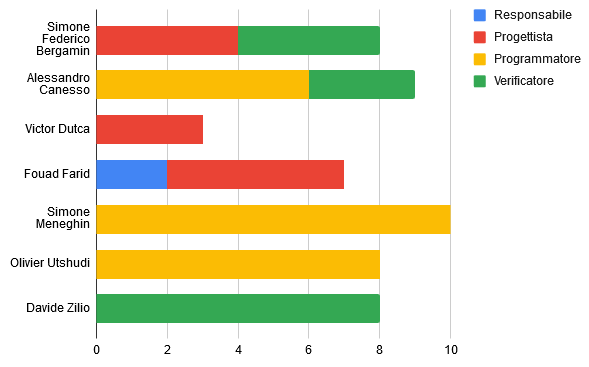
\includegraphics[scale=0.60]{img/grafici/tabella_inc12.png}
\caption{Istogramma della ripartizione delle ore per lo sviluppo dell'incremento 12}
\end{figure}

\subsubsection{Prospetto economico}
In questa fase il costo per ogni ruolo è il seguente:
 
%tabella costi
\begin{table}[H]
\centering\renewcommand{\arraystretch}{1.5}
\caption{Prospetto dei costi nella fase di Progettazione di dettaglio e codifica}
\vspace{0.2cm}
\begin{tabular}{ c c c }
\rowcolor{redafk}
\textcolor{white}{\textbf{Ruolo}} & \textcolor{white}{\textbf{Ore}} &
\textcolor{white}{\textbf{Costo}}  \\
Responsabile & 18 & 540€ \\
Amministratore & 23 & 460€ \\
Analista & 0 & 0€ \\
Progettista & 74 & 1628€ \\
Programmatore & 140 & 2100€  \\
Verificatore & 83 & 1245€  \\
\rowcolor{lastrowcolor}
\textbf{Totale} & \textbf{338} & \textbf{5973€}  \\
\end{tabular}
\end{table}
 
I dati ottenuti sono riassunti nel seguente areogramma:
\begin{figure}[H]
\centering
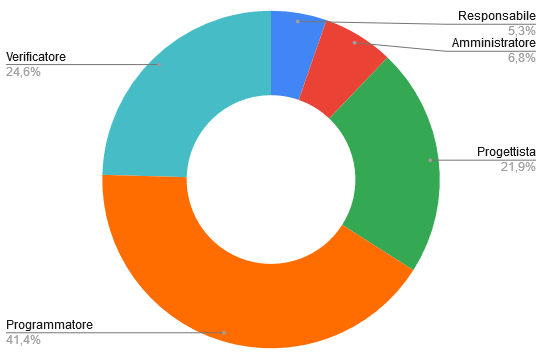
\includegraphics[scale=0.60]{img/grafici/torta_fase_prog_cod.png}
\caption{Areogramma della ripartizione dei costi per ruolo nella fase di Progettazione di dettaglio e codifica}
\end{figure}

\paragraph{Prospetto economico incrementi}
\paragraph*{Incremento 4}\mbox{} \\
\begin{table}[H]
\centering\renewcommand{\arraystretch}{1.5}
\caption{Prospetto dei costi per lo sviluppo dell'incremento 4}
\vspace{0.2cm}
\begin{tabular}{ c c c }
\rowcolor{redafk}
\textcolor{white}{\textbf{Ruolo}} & \textcolor{white}{\textbf{Ore}} &
\textcolor{white}{\textbf{Costo}}  \\
Responsabile & 2 & 60€ \\
Amministratore & 4 & 80€ \\
Analista & 0 & 0€ \\
Progettista & 4 & 88€ \\
Programmatore & 16 & 240€  \\
Verificatore & 6 & 90€  \\
\rowcolor{lastrowcolor}
\textbf{Totale} & \textbf{32} & \textbf{558€}  \\
\end{tabular}
\end{table}
 
I dati ottenuti sono riassunti nel seguente areogramma:
\begin{figure}[H]
\centering
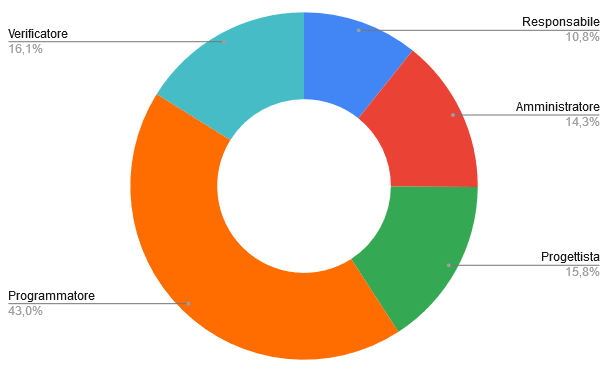
\includegraphics[scale=0.60]{img/grafici/torta_inc4.png}
\caption{Areogramma della ripartizione dei costi per ruolo per lo sviluppo dell'incremento 4}
\end{figure}

\paragraph*{Incremento 5}\mbox{} \\
\begin{table}[H]
\centering\renewcommand{\arraystretch}{1.5}
\caption{Prospetto dei costi per lo sviluppo dell'incremento 5}
\vspace{0.2cm}
\begin{tabular}{ c c c }
\rowcolor{redafk}
\textcolor{white}{\textbf{Ruolo}} & \textcolor{white}{\textbf{Ore}} &
\textcolor{white}{\textbf{Costo}}  \\
Responsabile & 1 & 30€ \\
Amministratore & 1 & 20€ \\
Analista & 0 & 0€ \\
Progettista & 1 & 22€ \\
Programmatore & 3 & 45€  \\
Verificatore & 2 & 30€  \\
\rowcolor{lastrowcolor}
\textbf{Totale} & \textbf{8} & \textbf{147€}  \\
\end{tabular}
\end{table}
 
I dati ottenuti sono riassunti nel seguente areogramma:
\begin{figure}[H]
\centering
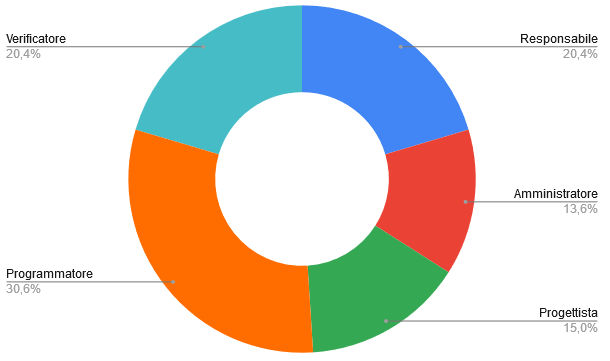
\includegraphics[scale=0.60]{img/grafici/torta_inc5.png}
\caption{Areogramma della ripartizione dei costi per ruolo per lo sviluppo dell'incremento 5}
\end{figure}

\paragraph*{Incremento 6}\mbox{} \\
\begin{table}[H]
\centering\renewcommand{\arraystretch}{1.5}
\caption{Prospetto dei costi per lo sviluppo dell'incremento 6}
\vspace{0.2cm}
\begin{tabular}{ c c c }
\rowcolor{redafk}
\textcolor{white}{\textbf{Ruolo}} & \textcolor{white}{\textbf{Ore}} &
\textcolor{white}{\textbf{Costo}}  \\
Responsabile & 3 & 90€ \\
Amministratore & 4 & 80€ \\
Analista & 0 & 0€ \\
Progettista & 6 & 132€ \\
Programmatore & 15 & 225€  \\
Verificatore & 6 & 90€  \\
\rowcolor{lastrowcolor}
\textbf{Totale} & \textbf{34} & \textbf{617€}  \\
\end{tabular}
\end{table}
 
I dati ottenuti sono riassunti nel seguente areogramma:
\begin{figure}[H]
\centering
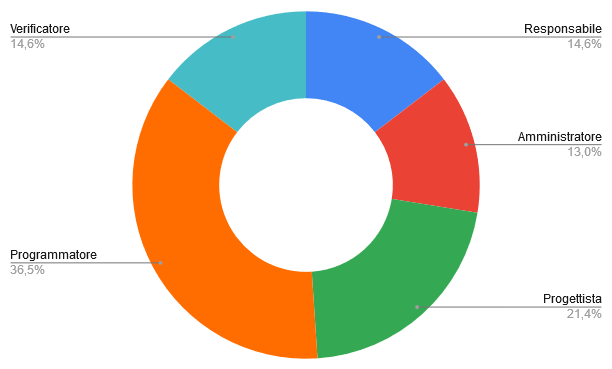
\includegraphics[scale=0.60]{img/grafici/torta_inc6.png}
\caption{Areogramma della ripartizione dei costi per ruolo per lo sviluppo dell'incremento 6}
\end{figure}

\paragraph*{Incremento 7}\mbox{} \\
\begin{table}[H]
\centering\renewcommand{\arraystretch}{1.5}
\caption{Prospetto dei costi per lo sviluppo dell'incremento 7}
\vspace{0.2cm}
\begin{tabular}{ c c c }
\rowcolor{redafk}
\textcolor{white}{\textbf{Ruolo}} & \textcolor{white}{\textbf{Ore}} &
\textcolor{white}{\textbf{Costo}}  \\
Responsabile & 2 & 60€ \\
Amministratore & 2 & 40€ \\
Analista & 0 & 0€ \\
Progettista & 10 & 220€ \\
Programmatore & 6 & 90€  \\
Verificatore & 4 & 60€  \\
\rowcolor{lastrowcolor}
\textbf{Totale} & \textbf{24} & \textbf{470€}  \\
\end{tabular}
\end{table}
 
I dati ottenuti sono riassunti nel seguente areogramma:
\begin{figure}[H]
\centering
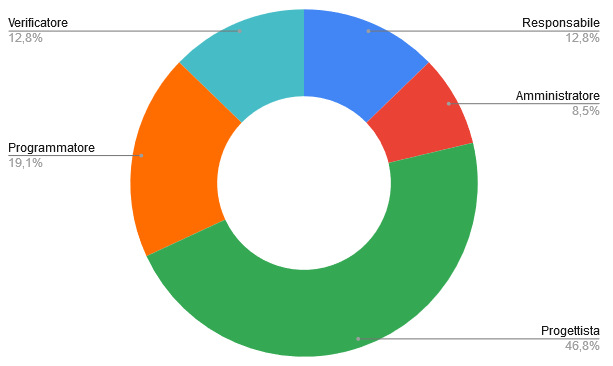
\includegraphics[scale=0.60]{img/grafici/torta_inc7.png}
\caption{Areogramma della ripartizione dei costi per ruolo per lo sviluppo dell'incremento 7}
\end{figure}

\paragraph*{Incremento 8}\mbox{} \\
\begin{table}[H]
\centering\renewcommand{\arraystretch}{1.5}
\caption{Prospetto dei costi per lo sviluppo dell'incremento 8}
\vspace{0.2cm}
\begin{tabular}{ c c c }
\rowcolor{redafk}
\textcolor{white}{\textbf{Ruolo}} & \textcolor{white}{\textbf{Ore}} &
\textcolor{white}{\textbf{Costo}}  \\
Responsabile & 3 & 90€ \\
Amministratore & 4 & 80€ \\
Analista & 0 & 0€ \\
Progettista & 8 & 176€ \\
Programmatore & 20 & 300€  \\
Verificatore & 11 & 165€  \\
\rowcolor{lastrowcolor}
\textbf{Totale} & \textbf{46} & \textbf{811€}  \\
\end{tabular}
\end{table}
 
I dati ottenuti sono riassunti nel seguente areogramma:
\begin{figure}[H]
\centering
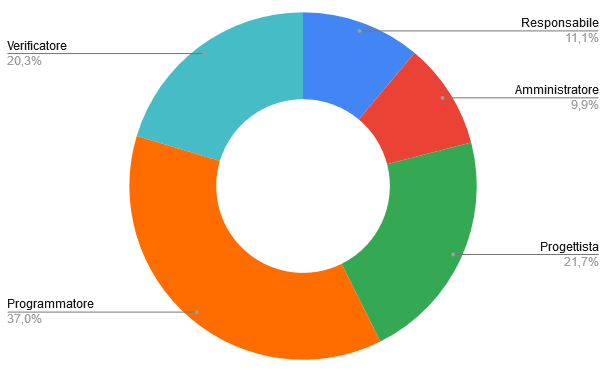
\includegraphics[scale=0.60]{img/grafici/torta_inc8.png}
\caption{Areogramma della ripartizione dei costi per ruolo per lo sviluppo dell'incremento 8}
\end{figure}

\paragraph*{Incremento 9}\mbox{} \\
\begin{table}[H]
\centering\renewcommand{\arraystretch}{1.5}
\caption{Prospetto dei costi per lo sviluppo dell'incremento 9}
\vspace{0.2cm}
\begin{tabular}{ c c c }
\rowcolor{redafk}
\textcolor{white}{\textbf{Ruolo}} & \textcolor{white}{\textbf{Ore}} &
\textcolor{white}{\textbf{Costo}}  \\
Responsabile & 2 & 60€ \\
Amministratore & 4 & 80€ \\
Analista & 0 & 0€ \\
Progettista & 15 & 330€ \\
Programmatore & 27 & 405€  \\
Verificatore & 20 & 300€  \\
\rowcolor{lastrowcolor}
\textbf{Totale} & \textbf{68} & \textbf{1175€}  \\
\end{tabular}
\end{table}
 
I dati ottenuti sono riassunti nel seguente areogramma:
\begin{figure}[H]
\centering
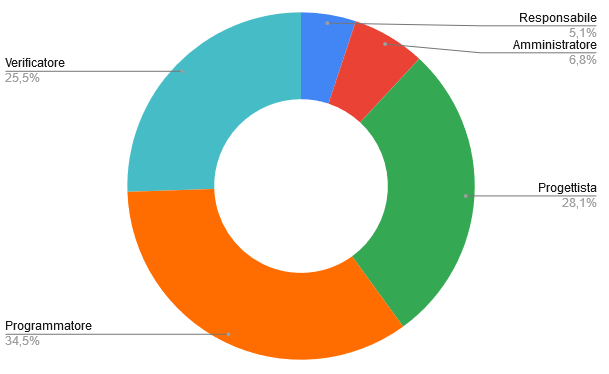
\includegraphics[scale=0.60]{img/grafici/torta_inc9.png}
\caption{Areogramma della ripartizione dei costi per ruolo per lo sviluppo dell'incremento 9}
\end{figure}

\paragraph*{Incremento 10}\mbox{} \\
\begin{table}[H]
\centering\renewcommand{\arraystretch}{1.5}
\caption{Prospetto dei costi per lo sviluppo dell'incremento 10}
\vspace{0.2cm}
\begin{tabular}{ c c c }
\rowcolor{redafk}
\textcolor{white}{\textbf{Ruolo}} & \textcolor{white}{\textbf{Ore}} &
\textcolor{white}{\textbf{Costo}}  \\
Responsabile & 1 & 30€ \\
Amministratore & 1 & 20€ \\
Analista & 0 & 0€ \\
Progettista & 7 & 154€ \\
Programmatore & 11 & 165€  \\
Verificatore & 9 & 135€  \\
\rowcolor{lastrowcolor}
\textbf{Totale} & \textbf{29} & \textbf{504€}  \\
\end{tabular}
\end{table}
 
I dati ottenuti sono riassunti nel seguente areogramma:
\begin{figure}[H]
\centering
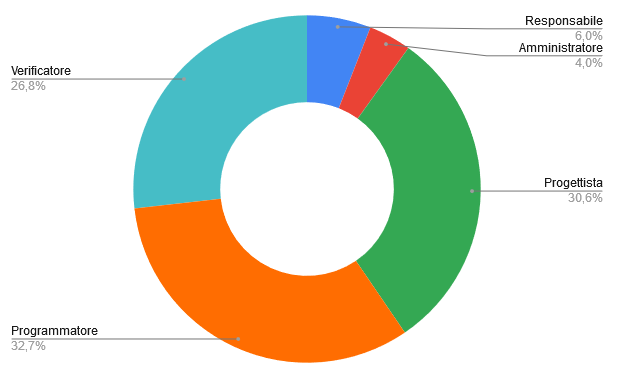
\includegraphics[scale=0.60]{img/grafici/torta_inc10.png}
\caption{Areogramma della ripartizione dei costi per ruolo per lo sviluppo dell'incremento 10}
\end{figure}

\paragraph*{Incremento 11}\mbox{} \\
\begin{table}[H]
\centering\renewcommand{\arraystretch}{1.5}
\caption{Prospetto dei costi per lo sviluppo dell'incremento 11}
\vspace{0.2cm}
\begin{tabular}{ c c c }
\rowcolor{redafk}
\textcolor{white}{\textbf{Ruolo}} & \textcolor{white}{\textbf{Ore}} &
\textcolor{white}{\textbf{Costo}}  \\
Responsabile & 2 & 60€ \\
Amministratore & 3 & 60€ \\
Analista & 0 & 0€ \\
Progettista & 11 & 242€ \\
Programmatore & 18 & 270€  \\
Verificatore & 10 & 150€  \\
\rowcolor{lastrowcolor}
\textbf{Totale} & \textbf{44} & \textbf{782€}  \\
\end{tabular}
\end{table}
 
I dati ottenuti sono riassunti nel seguente areogramma:
\begin{figure}[H]
\centering
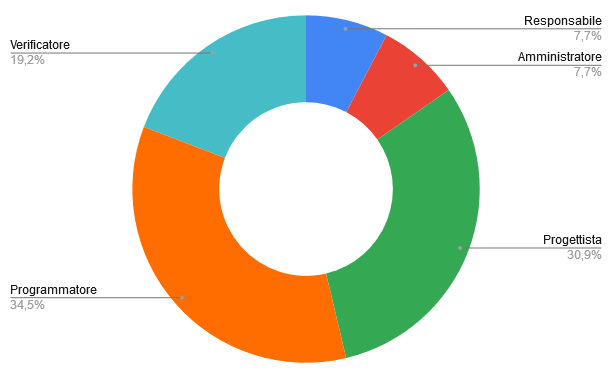
\includegraphics[scale=0.60]{img/grafici/torta_inc11.png}
\caption{Areogramma della ripartizione dei costi per ruolo per lo sviluppo dell'incremento 11}
\end{figure}

\paragraph*{Incremento 12}\mbox{} \\
\begin{table}[H]
\centering\renewcommand{\arraystretch}{1.5}
\caption{Prospetto dei costi per lo sviluppo dell'incremento 12}
\vspace{0.2cm}
\begin{tabular}{ c c c }
\rowcolor{redafk}
\textcolor{white}{\textbf{Ruolo}} & \textcolor{white}{\textbf{Ore}} &
\textcolor{white}{\textbf{Costo}}  \\
Responsabile & 2 & 60€ \\
Amministratore & 0 & 0€ \\
Analista & 0 & 0€ \\
Progettista & 12 & 264€ \\
Programmatore & 24 & 360€  \\
Verificatore & 15 & 225€  \\
\rowcolor{lastrowcolor}
\textbf{Totale} & \textbf{53} & \textbf{909€}  \\
\end{tabular}
\end{table}
 
I dati ottenuti sono riassunti nel seguente areogramma:
\begin{figure}[H]
\centering
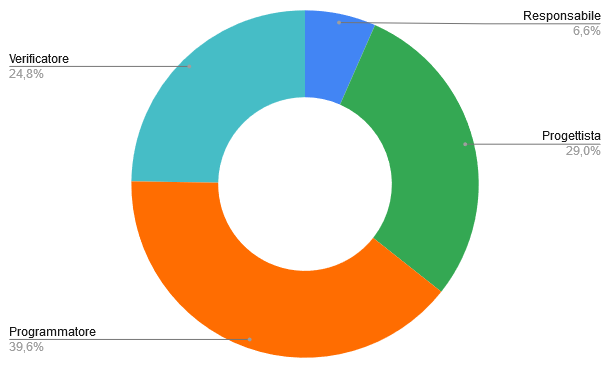
\includegraphics[scale=0.60]{img/grafici/torta_inc12.png}
\caption{Areogramma della ripartizione dei costi per ruolo per lo sviluppo dell'incremento 12}
\end{figure}

%------------------------------------

\subsection{Periodo di Validazione e collaudo}
\subsubsection{Distribuzione oraria}
In questa fase i ruoli sono così suddivisi:

%tabella ore
\begin{table}[H]
\centering\renewcommand{\arraystretch}{1.5}
\caption{Validazione e Collaudo}
\vspace{0.2cm}
\begin{tabular}{ c c c c c c c c }
\rowcolor{redafk}
\textcolor{white}{\textbf{Nominativo}} & \textcolor{white}{\textbf{Re}} & 
\textcolor{white}{\textbf{Am}} & \textcolor{white}{\textbf{An}} &
\textcolor{white}{\textbf{Pt}} & \textcolor{white}{\textbf{Pm}} &
\textcolor{white}{\textbf{Ve}} & \textcolor{white}{\textbf{Totale}} \\
Simone Federico Bergamin 	& 5 	& - 	& - 	& - 	& 8 	& 12 	& 25 \\
Alessandro Canesso 			& 4 	& 4 	& - 	& - 	& - 	& 15 	& 23 \\
Victor Dutca 				& 5 	& - 	& - 	& - 	& 5 	& 15 	& 25 \\
Fouad Farid					& - 	& 6 	& - 	& - 	& 7 	& 12 	& 25 \\
Simone Meneghin 			& - 	& 9 	& - 	& - 	& - 	& 16 	& 25 \\
Olivier Utshudi 			& - 	& 4 	& - 	& 4 	& 5 	& 12 	& 25 \\
Davide Zilio 				& 6 	& - 	& - 	& 8 	& - 	& 11 	& 25 \\
\rowcolor{lastrowcolor}
\textbf{Ore totali ruolo} & \textbf{20} & \textbf{23} & \textbf{0} & \textbf{12} & \textbf{25} & \textbf{93} & \textbf{173} \\
\end{tabular}
\end{table}

I dati ottenuti sono riassunti nel seguente istogramma: 
\begin{figure}[H]
\centering
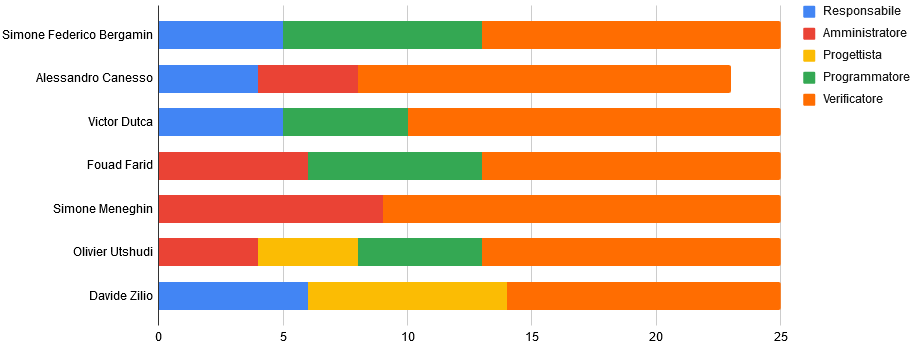
\includegraphics[scale=0.60]{img/grafici/tabella_fase_val_col.png}
\caption{Istogramma della ripartizione delle ore per ruolo nella fase di Validazione e collaudo}
\end{figure}

\paragraph{Distribuzione oraria incrementi}
\paragraph*{Incremento 13} \mbox{} \\
\begin{table}[H]
\centering\renewcommand{\arraystretch}{1.5}
\caption{Distribuzione delle ore per lo sviluppo dell'incremento 13}
\vspace{0.2cm}
\begin{tabular}{ c c c c c c c c }
\rowcolor{redafk}
\textcolor{white}{\textbf{Nominativo}} & \textcolor{white}{\textbf{Re}} &
\textcolor{white}{\textbf{Am}} & \textcolor{white}{\textbf{An}} &
\textcolor{white}{\textbf{Pt}} & \textcolor{white}{\textbf{Pm}} &
\textcolor{white}{\textbf{Ve}} & \textcolor{white}{\textbf{Totale}} \\
Simone Federico Bergamin & - & - & - & - & 2 & - & 2 \\
Alessandro Canesso & 2 & 1 & - & - & - & - & 3\\
Victor Dutca & - & - & - & - & - & - & 0 \\
Fouad Farid & - & - & - & - & - & 2 & 2 \\
Simone Meneghin & - & - & - & - & - & - & 0 \\
Olivier Utshudi & - & - & - & - & 2 & 3 & 5 \\
Davide Zilio & - & - & - & - & - & - & 0 \\
\rowcolor{lastrowcolor}
\textbf{Ore totali ruolo} & \textbf{2} & \textbf{1} & \textbf{0} & \textbf{2} & \textbf{5} & \textbf{2} & \textbf{12} \\
\end{tabular}
\end{table}

I dati ottenuti sono riassunti nel seguente istogramma:
\begin{figure}[H]
\centering
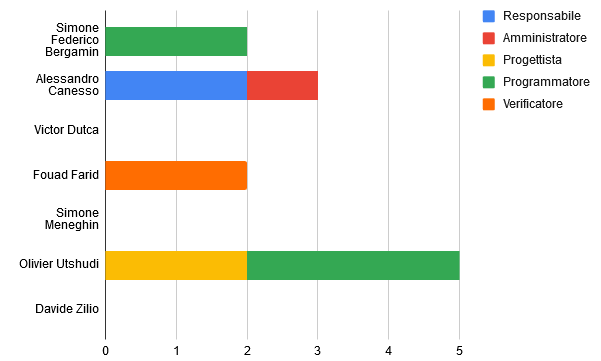
\includegraphics[scale=0.60]{img/grafici/tabella_inc13.png}
\caption{Istogramma della ripartizione delle ore per lo sviluppo dell'incremento 13}
\end{figure}

\paragraph*{Incremento 14} \mbox{} \\
\begin{table}[H]
\centering\renewcommand{\arraystretch}{1.5}
\caption{Distribuzione delle ore per lo sviluppo dell'incremento 14}
\vspace{0.2cm}
\begin{tabular}{ c c c c c c c c }
\rowcolor{redafk}
\textcolor{white}{\textbf{Nominativo}} & \textcolor{white}{\textbf{Re}} &
\textcolor{white}{\textbf{Am}} & \textcolor{white}{\textbf{An}} &
\textcolor{white}{\textbf{Pt}} & \textcolor{white}{\textbf{Pm}} &
\textcolor{white}{\textbf{Ve}} & \textcolor{white}{\textbf{Totale}} \\
Simone Federico Bergamin & - & - & - & - & - & - & 0 \\
Alessandro Canesso & 2 & 1 & - & - & - & - & 3\\
Victor Dutca & - & - & - & - & - & - & 0 \\
Fouad Farid & - & - & - & - & - & - & 0 \\
Simone Meneghin & - & - & - & - & - & - & 0 \\
Olivier Utshudi & - & - & - & 2 & 2 & - & 4 \\
Davide Zilio & - & - & - &- & - & 3 & 3 \\
\rowcolor{lastrowcolor}
\textbf{Ore totali ruolo} & \textbf{2} & \textbf{1} & \textbf{0} & \textbf{2} & \textbf{2} & \textbf{3} & \textbf{10} \\
\end{tabular}
\end{table}

I dati ottenuti sono riassunti nel seguente istogramma:
\begin{figure}[H]
\centering
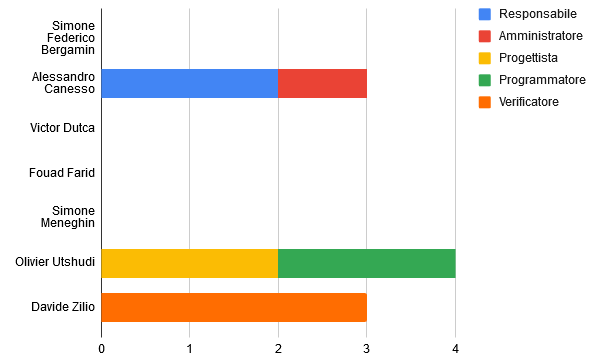
\includegraphics[scale=0.60]{img/grafici/tabella_inc14.png}
\caption{Istogramma della ripartizione delle ore per lo sviluppo dell'incremento 14}
\end{figure}

\paragraph{Distribuzione oraria sviluppo test per il collaudo del prodotto finale}\mbox{} \\
\begin{table}[H]
\centering\renewcommand{\arraystretch}{1.5}
\caption{Distribuzione delle ore per lo sviluppo e verifica dei test e del prodotto finale}
\vspace{0.2cm}
\begin{tabular}{ c c c c c c c c }
\rowcolor{redafk}
\textcolor{white}{\textbf{Nominativo}} & \textcolor{white}{\textbf{Re}} &
\textcolor{white}{\textbf{Am}} & \textcolor{white}{\textbf{An}} &
\textcolor{white}{\textbf{Pt}} & \textcolor{white}{\textbf{Pm}} &
\textcolor{white}{\textbf{Ve}} & \textcolor{white}{\textbf{Totale}} \\
Simone Federico Bergamin & 5 & - & - & - & 6 & 12 & 23 \\
Alessandro Canesso & - & 2 & - & - & - & 15 & 17\\
Victor Dutca & 5 & - & - & - & 5 & 15 & 25 \\
Fouad Farid & - & 6 & - & - & 7 & 10 & 23 \\
Simone Meneghin & - & 9 & - & - & - & 16 & 25 \\
Olivier Utshudi & - & 4 & - & - & - & 12 & 16 \\
Davide Zilio & 6 & - & - & 8 & - & 8 & 22 \\
\rowcolor{lastrowcolor}
\textbf{Ore totali ruolo} & \textbf{16} & \textbf{21} & \textbf{0} & \textbf{8} & \textbf{18} & \textbf{88} & \textbf{151} \\
\end{tabular}
\end{table}

I dati ottenuti sono riassunti nel seguente istogramma:
\begin{figure}[H]
\centering
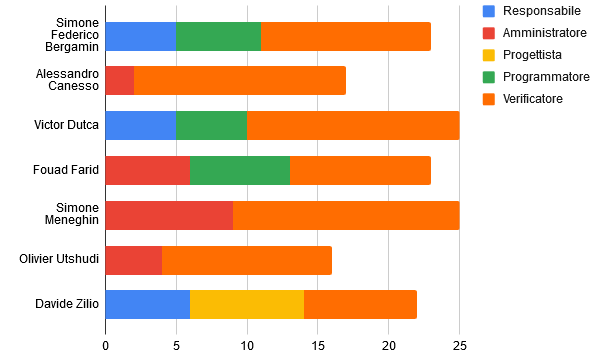
\includegraphics[scale=0.60]{img/grafici/tabella_test.png}
\caption{Istogramma della ripartizione delle ore per lo sviluppo e verifica dei test e del prodotto finale}
\end{figure}

\subsubsection{Prospetto economico}
In questa fase il costo per ogni ruolo è il seguente:

%tabella costi
\begin{table}[H]
\centering\renewcommand{\arraystretch}{1.5}
\caption{Prospetto dei costi nella fase di Validazione e collaudo}
\vspace{0.2cm}
\begin{tabular}{ c c c }
\rowcolor{redafk}
\textcolor{white}{\textbf{Ruolo}} & \textcolor{white}{\textbf{Ore}} & 
\textcolor{white}{\textbf{Costo}}  \\
Responsabile & 20 & 600€ \\
Amministratore & 23 & 460€ \\
Analista & - & - \\
Progettista	& 12 & 264€ \\
Programmatore & 25 & 375€  \\
Verificatore & 93 & 1395€  \\
\rowcolor{lastrowcolor}
\textbf{Totale} & \textbf{173} & \textbf{3094€}  \\
\end{tabular}
\end{table}

I dati ottenuti si possono riassumere nel seguente areogramma:
\begin{figure}[H]
\centering
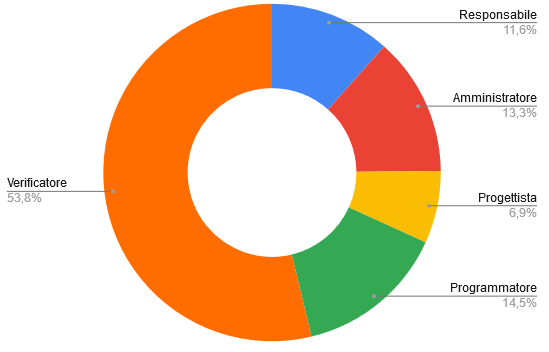
\includegraphics[scale=0.60]{img/grafici/torta_fase_val_col.png}
\caption{Areogramma della ripartizione dei costi per ruolo nella fase di Validazione e collaudo}
\end{figure}

\paragraph{Prospetto economico incrementi}
\paragraph*{Incremento 13}\mbox{} \\
\begin{table}[H]
\centering\renewcommand{\arraystretch}{1.5}
\caption{Prospetto dei costi per lo sviluppo dell'incremento 13}
\vspace{0.2cm}
\begin{tabular}{ c c c }
\rowcolor{redafk}
\textcolor{white}{\textbf{Ruolo}} & \textcolor{white}{\textbf{Ore}} &
\textcolor{white}{\textbf{Costo}}  \\
Responsabile & 2 & 60€ \\
Amministratore & 1 & 20€ \\
Analista & 0 & 0€ \\
Progettista & 2 & 44€ \\
Programmatore & 5 & 75€  \\
Verificatore & 2 & 30€  \\
\rowcolor{lastrowcolor}
\textbf{Totale} & \textbf{12} & \textbf{229€}  \\
\end{tabular}
\end{table}
 
I dati ottenuti sono riassunti nel seguente areogramma:
\begin{figure}[H]
\centering
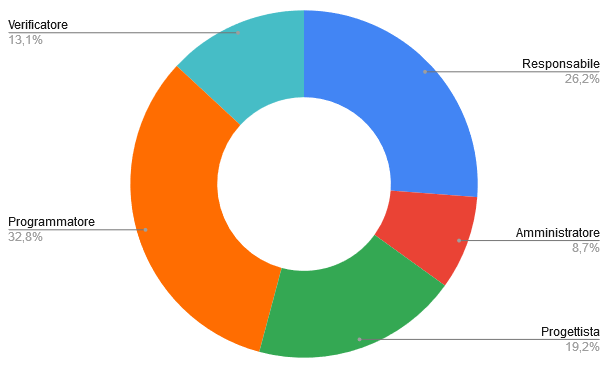
\includegraphics[scale=0.60]{img/grafici/torta_inc13.png}
\caption{Areogramma della ripartizione dei costi per ruolo per lo sviluppo dell'incremento 13}
\end{figure}

\paragraph*{Incremento 14}\mbox{} \\
\begin{table}[H]
\centering\renewcommand{\arraystretch}{1.5}
\caption{Prospetto dei costi per lo sviluppo dell'incremento 14}
\vspace{0.2cm}
\begin{tabular}{ c c c }
\rowcolor{redafk}
\textcolor{white}{\textbf{Ruolo}} & \textcolor{white}{\textbf{Ore}} &
\textcolor{white}{\textbf{Costo}}  \\
Responsabile & 2 & 60€ \\
Amministratore & 1 & 20€ \\
Analista & 0 & 0€ \\
Progettista & 2 & 44€ \\
Programmatore & 2 & 30€  \\
Verificatore & 3 & 45€  \\
\rowcolor{lastrowcolor}
\textbf{Totale} & \textbf{10} & \textbf{199€}  \\
\end{tabular}
\end{table}
 
I dati ottenuti sono riassunti nel seguente areogramma:
\begin{figure}[H]
\centering
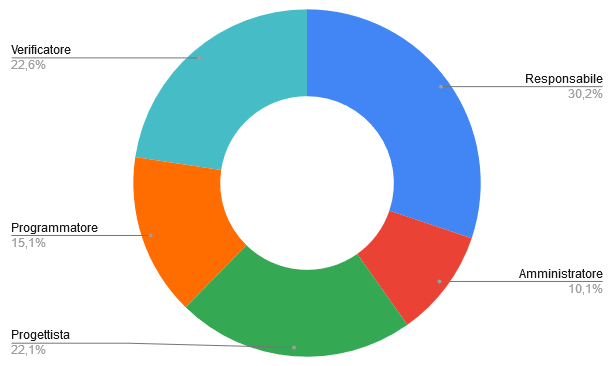
\includegraphics[scale=0.60]{img/grafici/torta_inc14.png}
\caption{Areogramma della ripartizione dei costi per ruolo per lo sviluppo dell'incremento 14}
\end{figure}

\paragraph{Prospetto economico sviluppo test per il collaudo del prodotto finale}\mbox{} \\
\begin{table}[H]
\centering\renewcommand{\arraystretch}{1.5}
\caption{Prospetto dei costi per lo sviluppo e verifica dei test e del prodotto finale}
\vspace{0.2cm}
\begin{tabular}{ c c c }
\rowcolor{redafk}
\textcolor{white}{\textbf{Ruolo}} & \textcolor{white}{\textbf{Ore}} &
\textcolor{white}{\textbf{Costo}}  \\
Responsabile & 16 & 480€ \\
Amministratore & 21 & 420€ \\
Analista & 0 & 0€ \\
Progettista & 8 & 176€ \\
Programmatore & 18 & 270€  \\
Verificatore & 88 & 1320€  \\
\rowcolor{lastrowcolor}
\textbf{Totale} & \textbf{151} & \textbf{2666€}  \\
\end{tabular}
\end{table}
 
I dati ottenuti sono riassunti nel seguente areogramma:
\begin{figure}[H]
\centering
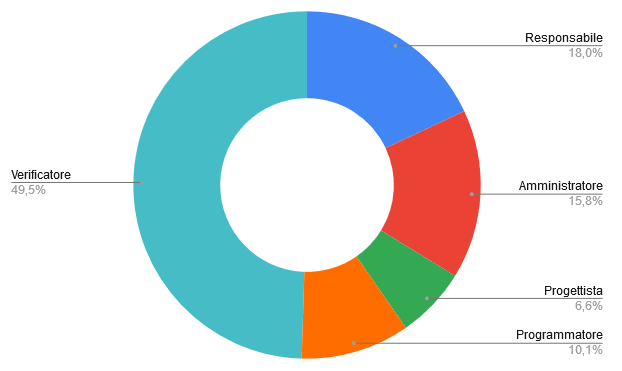
\includegraphics[scale=0.60]{img/grafici/torta_test.png}
\caption{Areogramma della ripartizione dei costi per ruolo per lo sviluppo e verifica dei test e del prodotto finale}
\end{figure}

\subsection{Riepilogo}
\subsubsection{Ore rendicontate con investimento}
\paragraph{Distribuzione oraria} \mbox{} \\ \mbox{} \\
Vengono riportate il totale delle ore del progetto in cui sono presenti le ore di investimento e le
ore rendicontate a carico del committente:

%tabella ore
\begin{table}[H]
\centering\renewcommand{\arraystretch}{1.5}
\caption{Distribuzione totale delle ore dell'intero progetto con investimento}
\vspace{0.2cm}
\begin{tabular}{ c c c c c c c c }
\rowcolor{redafk}
\textcolor{white}{\textbf{Nominativo}} & \textcolor{white}{\textbf{Re}} & 
\textcolor{white}{\textbf{Am}} & \textcolor{white}{\textbf{An}} &
\textcolor{white}{\textbf{Pt}} & \textcolor{white}{\textbf{Pm}} &
\textcolor{white}{\textbf{Ve}} & \textcolor{white}{\textbf{Totale}} \\
Simone Federico Bergamin 	& 11 	& 13 	& 30 	& 19 	& 31 	& 41 	& 145 \\
Alessandro Canesso 			& 16 	& 18 	& 16 	& 20 	& 27 	& 46 	& 143 \\
Victor Dutca 				& 17	& 14 	& 19 	& 20 	& 32 	& 41 	& 143 \\
Fouad Farid					& 11	& 18 	& 12 	& 32 	& 27 	& 43 	& 143 \\
Simone Meneghin 			& 8 	& 17 	& 22 	& 32 	& 28 	& 40 	& 147 \\
Olivier Utshudi 			& 8 	& 16 	& 13 	& 28 	& 33 	& 49 	& 147 \\
Davide Zilio 				& 13 	& 11 	& 30 	& 18 	& 20 	& 51 	& 143 \\
\rowcolor{lastrowcolor}
\textbf{Ore totali ruolo} & \textbf{84} & \textbf{107} & \textbf{142} & \textbf{169} & \textbf{198} & \textbf{311} & \textbf{1011} \\
\end{tabular}
\end{table}

Una rappresentazione visiva della suddivisione oraria viene data dal seguente grafico:
\begin{figure}[H]
\centering
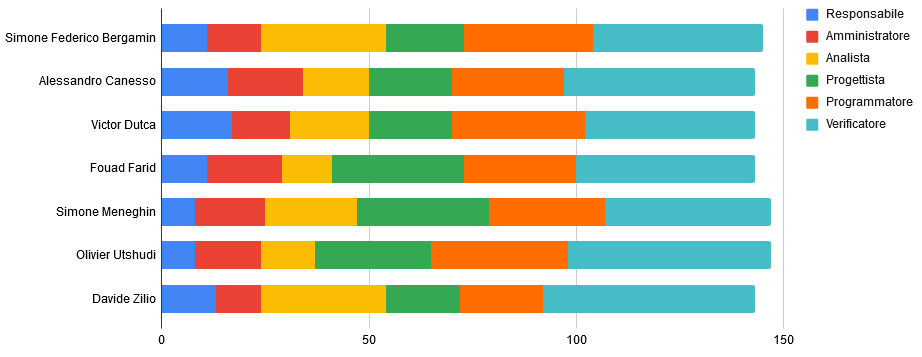
\includegraphics[scale=0.60]{img/grafici/tabella_tot_con_analisi.png}
\caption{Istogramma della ripartizione delle ore totali per ruolo con investimento}
\end{figure}

\paragraph{Prospetto economico} \mbox{} \\ \mbox{} \\
Il costo totale con investimento è riportato nella seguente tabella:

%tabella costi
\begin{table}[H]
\centering\renewcommand{\arraystretch}{1.5}
\caption{Costi totali con investimento}
\vspace{0.2cm}
\begin{tabular}{ c c c }
\rowcolor{redafk}
\textcolor{white}{\textbf{Ruolo}} & \textcolor{white}{\textbf{Ore}} & 
\textcolor{white}{\textbf{Costo}}  \\
Responsabile & 84 & 2520€ \\
Amministratore & 107 & 2140€ \\
Analista & 142 & 3550€ \\
Progettista	& 169 & 3718€ \\
Programmatore & 198 & 2970€  \\
Verificatore & 311 & 4665€  \\
\rowcolor{lastrowcolor}
\textbf{Totale} & \textbf{1011} & \textbf{19563€}  \\
\end{tabular}
\end{table}

I dati ottenuti si possono riassumere nel seguente areogramma:
\begin{figure}[H]
\centering
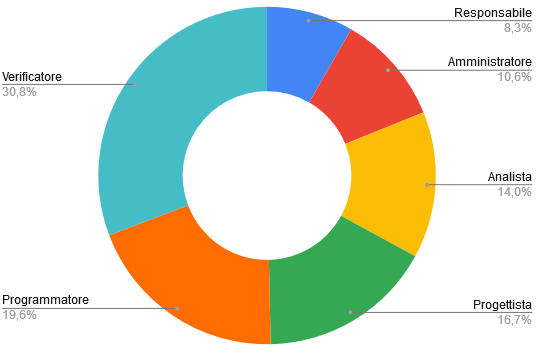
\includegraphics[scale=0.60]{img/grafici/torta_tot_con_analisi.png}
\caption{Areogramma della ripartizione dei costi totali per ruolo con investimento}
\end{figure}

\subsubsection{Ore rendicontate senza investimento}
\paragraph{Distribuzione oraria} \mbox{} \\ \mbox{} \\
Le ore rendicontate sono riassunte nella seguente tabella:

%tabella ore
\begin{table}[H]
\centering\renewcommand{\arraystretch}{1.5}
\caption{Distribuzione totale delle ore dell'intero progetto senza investimento}
\vspace{0.2cm}
\begin{tabular}{ c c c c c c c c }
\rowcolor{redafk}
\textcolor{white}{\textbf{Nominativo}} & \textcolor{white}{\textbf{Re}} & 
\textcolor{white}{\textbf{Am}} & \textcolor{white}{\textbf{An}} &
\textcolor{white}{\textbf{Pt}} & \textcolor{white}{\textbf{Pm}} &
\textcolor{white}{\textbf{Ve}} & \textcolor{white}{\textbf{Totale}} \\
Simone Federico Bergamin 	& 5 	& 6 	& 10	& 19	& 31	& 32 	& 103 \\
Alessandro Canesso 			& 8 	& 12	& - 	& 20	& 27	& 34 	& 101 \\
Victor Dutca 				& 8 	& 14	& 4 	& 20	& 32	& 25 	& 103 \\
Fouad Farid					& 4 	& 11	& - 	& 26	& 27	& 35 	& 103 \\
Simone Meneghin 			& 8 	& 9 	& 8 	& 22	& 28	& 30 	& 105 \\
Olivier Utshudi 			& 8 	& 8 	& - 	& 20	& 33	& 36 	& 105 \\
Davide Zilio 				& 9 	& 6 	& 13	& 18	& 20	& 37 	& 103 \\
\rowcolor{lastrowcolor}
\textbf{Ore totali ruolo} & \textbf{50} & \textbf{66} & \textbf{35} & \textbf{145} & \textbf{198} & \textbf{229} & \textbf{723} \\
\end{tabular}
\end{table}

Una rappresentazione visiva della suddivisione oraria viene data dal seguente grafico:
\begin{figure}[H]
\centering
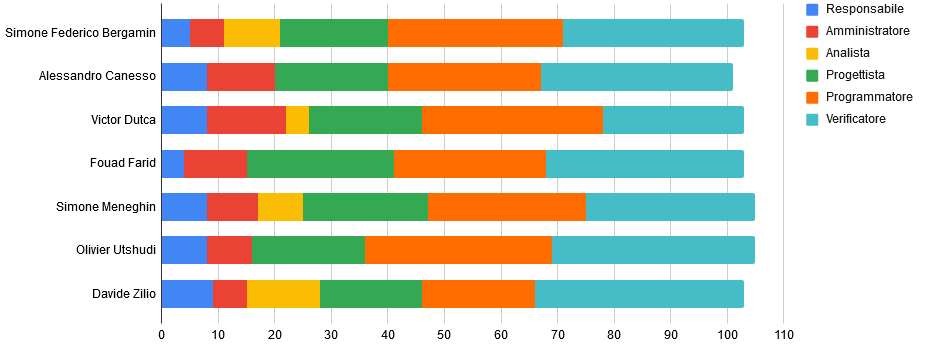
\includegraphics[scale=0.60]{img/grafici/tabella_tot_no_analisi.png}
\caption{Istogramma della ripartizione delle ore totali per ruolo con investimento}
\end{figure}

\paragraph{Prospetto economico} \mbox{} \\ \mbox{} \\
Il costo totale senza investimento è riportato nella seguente tabella:

%tabella costi
\begin{table}[H]
\centering\renewcommand{\arraystretch}{1.5}
\caption{Costi totali senza investimento}
\vspace{0.2cm}
\begin{tabular}{ c c c }
\rowcolor{redafk}
\textcolor{white}{\textbf{Ruolo}} & \textcolor{white}{\textbf{Ore}} & 
\textcolor{white}{\textbf{Costo}}  \\
Responsabile & 50 & 1500€ \\
Amministratore & 66 & 1320€ \\
Analista & 35 & 875€ \\
Progettista	& 145 & 3190€ \\
Programmatore & 198 & 2970€  \\
Verificatore & 229 & 3435€  \\
\rowcolor{lastrowcolor}
\textbf{Totale} & \textbf{723} & \textbf{13290€}  \\
\end{tabular}
\end{table}

I dati ottenuti si possono riassumere nel seguente areogramma:
\begin{figure}[H]
\centering
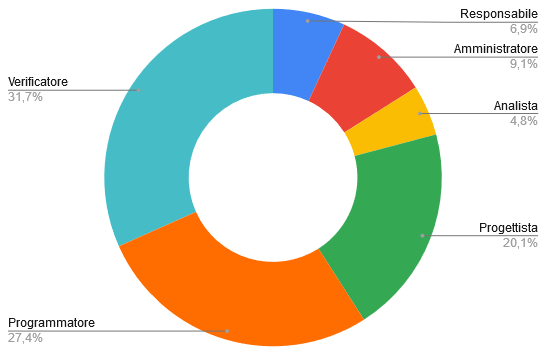
\includegraphics[scale=0.60]{img/grafici/torta_tot_no_analisi.png}
\caption{Areogramma della ripartizione dei costi totali per ruolo senza investimento}
\end{figure}

\subsection{Conclusioni}
Il costo totale preventivato per il progetto è 13.290,00€
\pagebreak

\section{Consuntivo di periodo}
Di seguito verranno indicate le spese effettivamente sostenute da ogni ruolo. Il bilancio di consuntivo potrà risultare: \begin{itemize}
\item \textbf{Positivo}: se il preventivo supera il consuntivo;
\item \textbf{Pari}: se preventivo e consuntivo sono uguali;
\item \textbf{Negativo}: se il consuntivo supera il preventivo.
\end{itemize}

\subsection{Analisi}
%tabella costi
\begin{table}[H]
\centering\renewcommand{\arraystretch}{1.5}
\caption{Consuntivo del periodo di Analisi}
\vspace{0.2cm}
\begin{tabular}{ c c c }
\rowcolor{redafk}
\textcolor{white}{\textbf{Ruolo}} & \textcolor{white}{\textbf{Ore}} & 
\textcolor{white}{\textbf{Costo}}  \\
Responsabile & 34 & 1020€ \\
Amministratore & 41 (+13) & 820€ (+260€) \\
Analista & 107 (+8) & 2675€ (+200€) \\
Progettista	& 24 & 528€  \\
Programmatore & 0 & 0€  \\
Verificatore & 82 (+9) & 1230€ (+135€)  \\
\textbf{Totale preventivo} & \textbf{288} & \textbf{6273€}  \\
\textbf{Totale consuntivo} & \textbf{318} & \textbf{6868€}  \\
\rowcolor{lastrowcolor}
\textbf{Differenza} & \textbf{+30} & \textbf{+595€}  \\
\end{tabular}
\end{table}

\subsubsection{Conclusioni}
Come emerge dai dati riportati nella tabella soprastante è stato necessario investire più tempo del previsto nei ruoli di \textit{Amministratore}, \textit{Analista} e \textit{Verificatore}. Per questo motivo il bilancio risultante è negativo. Le cause di tali ritardi sono riportate di seguito:
\begin{itemize}
\item \textbf{\textit{Amministratore}}: è servito più tempo del previsto per riuscire ad individuare i software più adatti per la gestione del progetto e per la loro  configurazione. Inoltre sono state aggiunte ed aggiornate alcune sezioni nelle \textit{Norme di Progetto}, necessarie al chiarimento di alcune problematiche sorte durante la stesura dei documenti;
\item \textbf{\textit{Analista}}: alcuni requisiti si sono rivelati di non facile comprensione, e sono state necessarie più ore di lavoro per la discussione interna tra gli \textit{Analisti} ed esterna con il proponente;
\item \textbf{\textit{Verificatore}}: l’aggiunta di nuove sezioni nelle \textit{Norme di Progetto} e l'inesperienza dei membri hanno implicato un maggiore lavoro anche per questo ruolo.
\end{itemize}
Il notevole quantitativo di ore che il gruppo ha dovuto impiegare nel primo periodo non deve ripetersi durante il lavoro rendicontato. Per le problematiche riscontrate verranno adottate le seguenti contromisure:
\begin{itemize}
	\item amministrazione degli strumenti: il gruppo ha ricercato e configurato in anticipo gli strumenti che verranno usati. In caso venissero individuati nuovi strumenti avere già un ambiente di sviluppo impostato correttamente per tutti i membri semplificherà la nuova configurazione e ridurrà l'insorgere di problemi;
	\item comprensione dei requisiti: i requisiti sono stati ampiamente discussi con il proponente durante questa fase, non si prevede di incorrere ulteriormente in tale problema;
	\item applicazione delle norme: i membri del gruppo hanno studiato attentamente le norme, in modo tale da poter redigere fin da subito nuove sezioni dei documenti già normate, semplificando il lavoro ai verificatori.
\end{itemize}

\subsubsection{Preventivo a finire}
Essendo questo periodo non rendicontato, non vengono a generarsi problemi nel monte ore totale, nonché nel preventivo economico. Nonostante ciò \textit{TeamAFK} si impegnerà a integrare altre misure di contenimento ad eventuali nuovi problemi, facendo esperienza dei problemi riscontrati durante questo primo periodo

\subsection{Progettazione e codifica per la Technology Baseline}

\begin{table}[H]
\centering\renewcommand{\arraystretch}{1.5}
\caption{Consuntivo del periodo di Progettazione e codifica per la Technology Baseline}
\vspace{0.2cm}
\begin{tabular}{ c c c }
\rowcolor{redafk}
\textcolor{white}{\textbf{Ruolo}} & \textcolor{white}{\textbf{Ore}} &
\textcolor{white}{\textbf{Costo}}  \\
Responsabile 	& 12 & 360€ \\
Amministratore 	& 20 (+9) 	& 400€ (+180€) \\
Analista 		& 35 (-20) 	& 875€ (-500€) \\
Progettista		& 59 (+8) 	& 1298€ (+176€)\\
Programmatore	& 33 (+13) 	& 495€ (+195€)\\
Verificatore 	& 53 & 795€ \\
\textbf{Totale preventivo} & \textbf{212} & \textbf{4223€}  \\
\textbf{Totale consuntivo} & \textbf{222} & \textbf{4274€}  \\
\rowcolor{lastrowcolor}
\textbf{Differenza} & \textbf{+10} & \textbf{+51€}  \\
\end{tabular}
\end{table}

\subsubsection{Analisi degli incrementi}
Al fine di garantire uno sviluppo del progetto congruo con quanto preventivato
nei tempi e nei costi, gli incrementi individuati nella pianificazione sono stati sviluppati in parallelo. Terminata la fase di codifica, si rilevano eventuali problemi riscontrati ed eventualmente si modifica e si dettaglia ulteriormente la pianificazione futura in modo da mitigare gli effetti di questi imprevisti.

\paragraph*{Incremento 1} \mbox{} \\ \mbox{} \\
Il tempo dedicato alla codifica di questo incremento e le risorse assegnategli sono risultati ben bilanciati. I programmatori dedicati sono riusciti a sviluppare quanto pianificato entro la scadenza prefissata. \\ 
Terminato il proprio compito, quest'ultimi si sono messi a disposizione dei propri colleghi.

\paragraph*{Incremento 2} \mbox{} \\ \mbox{} \\
La codifica di questo incremento ha avuto dei rallentamenti dovuti all'inesperienza dei programmatori con tale tecnologia unita alla scarsa documentazione fornita da Grafana. \\ Il \textit{TeamAFK} ha sfruttato questo periodo per incrementare le proprie conoscenze ed abilità in relazione all'ambiente di sviluppo e ai linguaggi di programmazione necessari allo sviluppo di tale e future funzionalità. 

\paragraph*{Incremento 3} \mbox{} \\ \mbox{} \\
La codifica di questo incremento, come per l'incremento 2, ha avuto dei rallentamenti dovuti all'inesperienza dei programmatori con tale tecnologia unita alla scarsa documentazione fornita da Grafana. \\ 
Il \textit{TeamAFK} ha pertanto sfruttato questo periodo per incrementare le proprie conoscenze ed abilità in relazione all'ambiente di sviluppo e ai linguaggi di programmazione necessari allo sviluppo di tale e future funzionalità.

\subsubsection{Conclusioni}
Come emerge dai dati riportati nella tabella soprastante è stato necessario investire più tempo nei ruoli di \textit{Amministratore}, \textit{Progettista} e \textit{Programmatore} mentre l'\textit{Analista} ha visto una riduzione delle sue ore. Le cause di tali scostamenti sono riportate di seguito:
\begin{itemize}
	\item \textbf{\textit{Amministratore}}: la causa di questo aumento di ore è dovuto all'aggiunta e modifica di alcune parti delle \textit{Norme di Progetto};
	\item \textbf{\textit{Analista}}: l'elevata comunicazione con il proponente nel periodo di analisi ha permesso un'ottima comprensione del prodotto da sviluppare, questo ha permesso di concentrarsi principalmente sulla correzione dell'\textit{Analisi dei Requisiti};
	\item \textbf{\textit{Progettista}}: le ore aggiuntive sono state richieste per la correzione del documento \textit{Priano di Qualifica};
	\item \textbf{\textit{Programmatore}}: data l'inesperienza con le tecnologie utilizzate per lo sviluppo del software, sono state richieste più ore di programmazione per comprendere e quindi correggere i problemi che si sono presentati durante la codifica delle funzionalità previste per la PoC.
\end{itemize}

Rispetto alla fase di analisi, le ore aggiunte sono decisamente ridotte, però in questo caso le ore sono rendicontate, quindi lo sforamento è ben più grave. Per le problematiche riscontrate verranno adottate le seguenti contromisure: 
\begin{itemize}
	\item mancanza ed errata stesura di alcune sezioni delle norme: è stata prestata particolare attenzione durante la correzione, in modo tale che non si debbano correggere ulteriormente le \textit{Norme di Progetto} in futuro;
	\item correzione dei documenti: durante la stesura e la verifica si è stati più meticolosi, così da ridurre il più possibile eventuali nuove correzioni;
	\item inesperienza tecnologica: durante questa fase si è analizzato le componenti del prodotto che potrebbero essere più complicate, ricercando in anticipo informazioni ed possibili soluzioni.
\end{itemize}

\subsubsection{Preventivo a finire}
Il bilancio risultante è negativo, in quanto sono stati spesi 51€ in più rispetto a quanto preventivato. Per questo motivo sarà necessario impegnarsi per ridurre il costo dei successivi periodi senza però intaccare la qualità del prodotto finale.

\subsection{Periodo di progettazione di dettaglio e codifica}
\begin{table}[H]
\centering\renewcommand{\arraystretch}{1.5}
\caption{Consuntivo del periodo di progettazione di dettaglio e codifica}
\vspace{0.2cm}
\begin{tabular}{ c c c }
\rowcolor{redafk}
\textcolor{white}{\textbf{Ruolo}} & \textcolor{white}{\textbf{Ore}} &
\textcolor{white}{\textbf{Costo}}  \\
Responsabile 	& 18 & 540€ \\
Amministratore 	&  23	& 460€ \\
Analista 		& 0 (+6)  & 0 (+150€) \\
Progettista		&  74 (-8) & 1628€ (-176€)\\
Programmatore	&  	140 (-4)& 2100€ (-60€)\\
Verificatore 	& 83 (+2) &  1245€ (+30€)\\
\textbf{Totale preventivo} & \textbf{338} & \textbf{5973€}  \\
\textbf{Totale consuntivo} & \textbf{334} & \textbf{5917€} \\
\rowcolor{lastrowcolor}
\textbf{Differenza} & \textbf{-4} & \textbf{-56€} \\
\end{tabular}
\end{table}

\subsubsection{Analisi degli incrementi}
Di seguito sono analizzati tutti gli incrementi singolarmente, ed ognuno contiene una breve descrizione dei costi, negativi o positivi, presenti nella tabella.

\paragraph*{Incremento 4} \mbox{} \\ \mbox{} \\
Come riportato nella tabella seguente, la codifica di questo incremento ha richiesto meno tempo di quello preventivato, in quanto i \textit{Programmatori} avevano acquisito le conoscenze necessarie allo sviluppo di quest'ultimo nella fase precedente di Progettazione e codifica per la Technology Baseline (in particolare durante lo sviluppo dell'incremento 1). Sono state apportate inoltre delle piccole modifiche alla struttura del codice.
\begin{table}[H]
\centering\renewcommand{\arraystretch}{1.5}
\caption{Consuntivo dell'incremento 4}
\vspace{0.2cm}
\begin{tabular}{ c c c }
\rowcolor{redafk}
\textcolor{white}{\textbf{Ruolo}} & \textcolor{white}{\textbf{Ore}} &
\textcolor{white}{\textbf{Costo}}  \\
Responsabile 	& 2 & 60€ \\
Amministratore 	&  4 & 80€ \\
Analista 		&  0 & 0€ \\
Progettista		&  4 (-1) & 88€ (-22€)\\
Programmatore	&  14 (-2) & 240€ (-30€)\\
Verificatore 	& 6 & 90€ \\
\textbf{Totale preventivo} & \textbf{32} & \textbf{558€}  \\
\textbf{Totale consuntivo} & \textbf{29} & \textbf{506€}  \\
\rowcolor{lastrowcolor}
\textbf{Differenza} & \textbf{-3} & \textbf{-52€} \\
\end{tabular}
\end{table}

\paragraph*{Incremento 5} \mbox{} \\ \mbox{} \\
Come riportato nella tabella seguente, la codifica di questo incremento ha rispettato le tempistiche e i costi preventivati.
\begin{table}[H]
\centering\renewcommand{\arraystretch}{1.5}
\caption{Consuntivo dell'incremento 5}
\vspace{0.2cm}
\begin{tabular}{ c c c }
\rowcolor{redafk}
\textcolor{white}{\textbf{Ruolo}} & \textcolor{white}{\textbf{Ore}} &
\textcolor{white}{\textbf{Costo}}  \\
Responsabile 	& 1 & 30€ \\
Amministratore 	& 1 & 20€ \\
Analista 		& 0 & 0€ \\
Progettista		& 1 & 22€ \\
Programmatore	& 3 & 45€ \\
Verificatore 	& 2 & 30€ \\
\textbf{Totale preventivo} & \textbf{8} & \textbf{147€}  \\
\textbf{Totale consuntivo} & \textbf{8} & \textbf{147€}  \\
\rowcolor{lastrowcolor}
\textbf{Differenza} & \textbf{0} & \textbf{0€} \\
\end{tabular}
\end{table}

\paragraph*{Incremento 6} \mbox{} \\ \mbox{} \\
Come riportato nella tabella seguente, la codifica di questo incremento ha subito una leggera variazione, positiva, in quanto è stato implementato quanto necessario leggermente più velocemente rispetto a quanto pianificato.
\begin{table}[H]
\centering\renewcommand{\arraystretch}{1.5}
\caption{Consuntivo dell'incremento 6}
\vspace{0.2cm}
\begin{tabular}{ c c c }
\rowcolor{redafk}
\textcolor{white}{\textbf{Ruolo}} & \textcolor{white}{\textbf{Ore}} &
\textcolor{white}{\textbf{Costo}}  \\
Responsabile 	& 3 & 90€ \\
Amministratore 	& 4 & 80€ \\
Analista 		& 0  & 0€ \\
Progettista		& 6  &  132€\\
Programmatore	& 14 & 225€ (-15€) \\
Verificatore 	& 6 & 90€ \\
\textbf{Totale preventivo} & \textbf{34} & \textbf{617€}   \\
\textbf{Totale consuntivo} & \textbf{33} & \textbf{602€}  \\
\rowcolor{lastrowcolor}
\textbf{Differenza} & \textbf{-1} & \textbf{-15€} \\
\end{tabular}
\end{table}

\paragraph*{Incremento 7} \mbox{} \\ \mbox{} \\
Come riportato nella tabella seguente, la codifica di questo incremento ha richiesto meno ore di progettazione, in quanto l'architettura necessaria al suo sviluppo è stata ben definita dai \textit{Progettisti} e i \textit{Programmatori} non hanno avuto necessità di chiedere maggiori informazioni.
\begin{table}[H]
\centering\renewcommand{\arraystretch}{1.5}
\caption{Consuntivo dell'incremento 7}
\vspace{0.2cm}
\begin{tabular}{ c c c }
\rowcolor{redafk}
\textcolor{white}{\textbf{Ruolo}} & \textcolor{white}{\textbf{Ore}} &
\textcolor{white}{\textbf{Costo}}  \\
Responsabile 	& 2 & 60€ \\
Amministratore 	& 2 &  40€ \\
Analista 		& 0  & 0€ \\
Progettista		& 10 (-2)  & 220€ (-44€) \\
Programmatore	&  6 & 90€ \\
Verificatore 	&  4 & 60€ \\
\textbf{Totale preventivo} & \textbf{24} & \textbf{470€}  \\
\textbf{Totale consuntivo} & \textbf{22} & \textbf{426€}  \\
\rowcolor{lastrowcolor}
\textbf{Differenza} & \textbf{-2} & \textbf{-44€} \\
\end{tabular}
\end{table}

\paragraph*{Incremento 8} \mbox{} \\ \mbox{} \\
Come riportato nella tabella seguente, la codifica di questo incremento ha richiesto piu soldi (e ore) di quanto preventivato, in quanto sono stati riscontrati dei problemi nell'\textit{Analisi dei Requisiti}, da risolvere subito e nel minor tempo possibile. Tal'ultimi hanno richiesto 6 ore di analisi in più di quanto preventivato inizialmente.\\
La progettazione, invece, ha richiesto 1 ora in meno per mettere a punto e sviluppare l'idea architetturale dietro a questo incremento.
\begin{table}[H]
\centering\renewcommand{\arraystretch}{1.5}
\caption{Consuntivo dell'incremento 8}
\vspace{0.2cm}
\begin{tabular}{ c c c }
\rowcolor{redafk}
\textcolor{white}{\textbf{Ruolo}} & \textcolor{white}{\textbf{Ore}} &
\textcolor{white}{\textbf{Costo}}  \\
Responsabile 	& 3 & 90€ \\
Amministratore 	& 4 & 80€ \\
Analista 		& 0 (+6)  & 0 (+150€) \\
Progettista		& 8 (-1)  & 176€ (-22€) \\
Programmatore	& 20 & 300€ \\
Verificatore 	& 11 & 165€  \\
\textbf{Totale preventivo} & \textbf{46} & \textbf{811€}  \\
\textbf{Totale consuntivo} & \textbf{51} & \textbf{939€} \\
\rowcolor{lastrowcolor}
\textbf{Differenza} & \textbf{+5} & \textbf{+128€} \\
\end{tabular}
\end{table}

\paragraph*{Incremento 9} \mbox{} \\ \mbox{} \\
Come riportato nella tabella seguente, la codifica di questo incremento ha richiesto meno ore di progettazione, in quanto la sua struttura era già ben definita. 
\begin{table}[H]
\centering\renewcommand{\arraystretch}{1.5}
\caption{Consuntivo dell'incremento 9}
\vspace{0.2cm}
\begin{tabular}{ c c c }
\rowcolor{redafk}
\textcolor{white}{\textbf{Ruolo}} & \textcolor{white}{\textbf{Ore}} &
\textcolor{white}{\textbf{Costo}}  \\
Responsabile 	& 2 & 60€ \\
Amministratore 	& 4 & 80€ \\
Analista 		&  0 & 0€ \\
Progettista		&  15 (-4) & 330€ (-88€) \\
Programmatore	&  27 (-1) & 405€ (-15€) \\
Verificatore 	&  20 & 300€ \\
\textbf{Totale preventivo} & \textbf{68} & \textbf{1175€}  \\
\textbf{Totale consuntivo} & \textbf{63} & \textbf{1072€}  \\
\rowcolor{lastrowcolor}
\textbf{Differenza} & \textbf{-5} & \textbf{-103€} \\
\end{tabular}
\end{table}

\paragraph*{Incremento 10} \mbox{} \\ \mbox{} \\
Come riportato nella tabella seguente, la codifica di questo incremento ha rispetto quanto preventivato.
\begin{table}[H]
\centering\renewcommand{\arraystretch}{1.5}
\caption{Consuntivo dell'incremento 1o}
\vspace{0.2cm}
\begin{tabular}{ c c c }
\rowcolor{redafk}
\textcolor{white}{\textbf{Ruolo}} & \textcolor{white}{\textbf{Ore}} &
\textcolor{white}{\textbf{Costo}}  \\
Responsabile 	& 1 & 30€ \\
Amministratore 	& 1 & 20€ \\
Analista 		& 0 & 0€ \\
Progettista		& 7 & 154€ \\
Programmatore	& 11 & 165€\\
Verificatore 	& 9 &  135€\\
\textbf{Totale preventivo} & \textbf{29} & \textbf{504€}  \\
\textbf{Totale consuntivo} & \textbf{29} & \textbf{504€}  \\
\rowcolor{lastrowcolor}
\textbf{Differenza} & \textbf{0} & \textbf{0€} \\
\end{tabular}
\end{table}

\paragraph*{Incremento 11} \mbox{} \\ \mbox{} \\
Come riportato nella tabella seguente, la codifica di questo incremento ha richiesto due ore in più di verifica in quanto lo sviluppo di alcuni test ha richiesto più tempo del previsto data l'inesperienza del \textit{TeamAFK} con questo tipologia di codifica.
\begin{table}[H]
\centering\renewcommand{\arraystretch}{1.5}
\caption{Consuntivo dell'incremento 11}
\vspace{0.2cm}
\begin{tabular}{ c c c }
\rowcolor{redafk}
\textcolor{white}{\textbf{Ruolo}} & \textcolor{white}{\textbf{Ore}} &
\textcolor{white}{\textbf{Costo}}  \\
Responsabile 	& 2 & 60€  \\
Amministratore 	& 3	& 60€\\
Analista 		& 0  & 0€ \\
Progettista		& 11 & 242€ \\
Programmatore	& 18 & 270€ \\
Verificatore 	& 12 (+2) & 150€ (+30€) \\
\textbf{Totale preventivo} & \textbf{44} & \textbf{782€}  \\
\textbf{Totale consuntivo} & \textbf{46} & \textbf{812€}  \\
\rowcolor{lastrowcolor}
\textbf{Differenza} & \textbf{+2} & \textbf{+30€} \\
\end{tabular}
\end{table}

\paragraph*{Incremento 12} \mbox{} \\ \mbox{} \\
Come riportato nella tabella seguente, la codifica di questo incremento ha rispetto quanto preventivato.
\begin{table}[H]
\centering\renewcommand{\arraystretch}{1.5}
\caption{Consuntivo dell'incremento 12}
\vspace{0.2cm}
\begin{tabular}{ c c c }
\rowcolor{redafk}
\textcolor{white}{\textbf{Ruolo}} & \textcolor{white}{\textbf{Ore}} &
\textcolor{white}{\textbf{Costo}}  \\
Responsabile 	& 2 & 60€ \\
Amministratore 	& 0 & 0€ \\
Analista 		&  0 & 0€ \\
Progettista		&  12 & 264€ \\
Programmatore	&  24 & 360€ \\
Verificatore 	&  15 & 225€ \\
\textbf{Totale preventivo} & \textbf{53} & \textbf{909€}  \\
\textbf{Totale consuntivo} & \textbf{53} & \textbf{909€}  \\
\rowcolor{lastrowcolor}
\textbf{Differenza} & \textbf{0} & \textbf{0€} \\
\end{tabular}
\end{table}


\subsubsection{Conclusioni generali}
Come emerge dai dati riportati nella tabella è stato necessario investire più tempo nei ruoli di \textit{Analista} e \textit{Verificatore} mentre il \textit{Programmatore} e il \textit{Progettista} hanno visto una riduzione delle loro ore. Le cause di tali scostamenti sono riportate di seguito:
\begin{itemize}
	\item \textbf{\textit{Analista}}: è stato necessario rivedere la struttura dei casi d'uso e l'importanza di alcuni requisiti, in modo da soddisfare e rispettare il \textit{Piano di Progetto}. Infine, sono state apportate le correzioni indicate dal committente;
	\item \textbf{\textit{Progettista}}: i \textit{Progettisti} avevano studiato, descritto e impostato in modo esaustivo l'architettura del prodotto nella fase precedente; è stato richiesto quindi meno tempo per progettare quanto codificato e mostrato durante la Product Baseline e la Revisione di Qualifica; 
	\item \textbf{\textit{Programmatore}}: sono state richieste meno ore di programmazione per sviluppare quanto descritto in questo documento, data l'esperienza acquisita durante la Technology Baseline;
	\item \textbf{\textit{Verificatore}}: sono state richieste più ore di verifica, in quanto sono stati riscontrati dei problemi nella stesura dei test; nessun membro del \textit{TeamAFK} aveva esperienza con questo tipo di codifica.
\end{itemize}
Rispetto alla fase di Progettazione e codifica per la Technology Baseline, le ore aggiunte sono dovute principalmente all'inesperienza del \textit{TeamAFK} nella stesura di codice di test. \\
Per le problematiche riscontrate verranno adottate le seguenti contromisure: 
\begin{itemize}
	\item correzione dei documenti: durante la stesura e la verifica si è stati più meticolosi, così da ridurre il più possibile eventuali nuove correzioni;
	\item inesperienza tecnologica: questo periodo ha permesso al \textit{TeamAFK} di sviluppare nuove conoscenze. Quest'ultime velocizzeranno il processo di codifica del periodo successivo, in cui il progetto dovrà essere terminato del tutto.
\end{itemize}


\subsubsection{Preventivo a finire generale}
Le modifiche apportate alla pianificazione ci hanno permesso di avere un
bilancio positivo. Tale bilancio risulta tale in quanto i costi che abbiamo effettivamente rilevato sono inferiori a quelli che erano stati preventivati (-56€). Questi soldi risparmiati vengono utilizzati per coprire le spese in eccesso del periodo precedente.\\
Per quanto riguarda lo sviluppo degli incrementi, il \textit{TeamAFK} si ritiene soddisfatto di quanto prodotto in questo periodo.
\pagebreak

\appendix
\section{Riscontro dei rischi}
Di seguito vengono riportati i rischi in cui il gruppo si è imbattuto durante lo svolgimento del progetto, suddivisi per periodi.

\subsection{Rischi nella fase di Analisi}
I seguenti rischi sono stati riscontrati durante il periodo di analisi. \\
\textit{Periodo: da 2020-03-16 a 2020-04-13}

\begin{longtable}{C{3cm} L{5cm} L{7cm}}
\rowcolor{white}\caption{Attualizzazione dei rischi - Analisi} \\
		\rowcolor{redafk}
\textcolor{white}{\textbf{Rischio}} &
\textcolor{white}{\textbf{Descrizione}} &
\textcolor{white}{\textbf{Contromisura}}\\
		\endfirsthead
		\rowcolor{white}\caption[]{(continua)} \\
		\rowcolor{redafk}
\textcolor{white}{\textbf{Rischio}} &
\textcolor{white}{\textbf{Descrizione}} &
\textcolor{white}{\textbf{Contromisura}}\\
		\endhead

RiO01 - Emergenza sanitaria	& L'epidemia ha costretto gli stakeholders ad attuare lo smart working. & Sono stati usati vari mezzi di comunicazione, in particolare si ha optato per applicazioni che permettessero comunicazioni rapide e già conosciute così da ridurre il disagio al minimo.
\\
RiO06 - Divisione errata del lavoro & Durante la suddivisione dei compiti alcuni sono stati sottovalutati. & Il responsabile, una volta informato sugli errori di valutazione,ha proceduto ad individuare una migliore suddivisione. Per ridurre l'occorrenza di questo rischio il gruppo cercherà di fare spesso incontri di pochi minuti in cui discutere l'avanzamento del proprio compito e la necessità o possibilità di ricevere o dare aiuti.
\\
RiO07 - Errata analisi dei requisiti & Durante l'analisi sono sorti alcuni dubbi sui requisiti esposti dal proponente. & Il gruppo ha proceduto ad effettuare degli incontri con il proponente per poter chiarire tutti i dubbi rilevati.
\\

\end{longtable}


\subsection{Rischi nella fase di Progettazione e codifica per la Technology Baseline}
I seguenti rischi sono stati riscontrati durante il periodo di progettazione e codifica per la Technology Baseline. \\
\textit{Periodo: da 2020-04-21 a 2020-05-11}


\begin{longtable}{C{3cm} L{5cm} L{7cm}}
\rowcolor{white}\caption{Attualizzazione dei rischi - Progettazione e codifica per la Technology Baseline} \\
		\rowcolor{redafk}
\textcolor{white}{\textbf{Rischio}} &
\textcolor{white}{\textbf{Descrizione}} &
\textcolor{white}{\textbf{Contromisura}}\\
		\endfirsthead
		\rowcolor{white}\caption[]{(continua)} \\
		\rowcolor{redafk}
\textcolor{white}{\textbf{Rischio}} &
\textcolor{white}{\textbf{Descrizione}} &
\textcolor{white}{\textbf{Contromisura}}\\
		\endhead

RiT01 - Inesperienza tecnologica & I programmatori non conoscevano a pieno i linguaggi e le librerie che sono state utilizzate & \'E stato suddiviso il lavoro in modo da rispettare le conoscenze dei membri. In caso di nessuna conoscenza precedente, si è suddiviso il compito di studiare le documentazioni, per poi spiegarle agli altri membri.
\\
RiT04 - Configurazione dell'ambiente di lavoro & Alcuni membri con SO\glo Unix/Linux hanno riscontrato problemi nel far individuare a Grafana il plugin di test che era stato creato. & Si è consultata a fondo la documentazione individuando così le impostazioni da cambiare.
\\
RiT02 - Errori nelle dipendenze & Un cambiamento all'interno degli strumenti forniti da Grafana per sviluppare il plugin ha causato l'impossibilità di effettuare la build del prodotto. & Si è proceduto al passaggio ad una versione precedente di tali strumenti.
\\
RiO01 - Emergenza sanitaria	& L'epidemia ha costretto gli stakeholders ad attuare lo smart working. & Sono stati usati vari mezzi di comunicazione, in particolare si ha optato per applicazioni che permettessero comunicazioni rapide e già conosciute così da ridurre il disagio al minimo.
\\
RiO03 - Impegni accademici & Un membro del gruppo ha dovuto svolgere un esame & Durante la breve mancanza di un membro il resto del gruppo si è dedicato all'approfondimento e allo studio delle tecnologie utilizzate.
\\
RiO08 - Suddivisione delle ore di lavoro & La suddivisione delle ore per questa fase non è stata rispettata totalmente & Sono stati riscontrati problemi principalmente nelle ore di programmazione, ogni membro è stato informato dei problemi riscontrati e della loro soluzione in modo tale da evitare il loro ripresentarsi nelle fasi successive, evitando così di rallentare ulteriormente il lavoro.
\\

\end{longtable}


\subsection{Rischi nella fase di Progettazione di dettaglio e codifica}
I seguenti rischi sono stati riscontrati durante il periodo di progettazione di dettaglio e codifica. \\
\textit{Periodo: da 2020-05-11 a 2020-06-11}


\begin{longtable}{C{3cm} L{5cm} L{7cm}}
\rowcolor{white}\caption{Attualizzazione dei rischi - Progettazione di dettaglio e codifica} \\
		\rowcolor{redafk}
\textcolor{white}{\textbf{Rischio}} &
\textcolor{white}{\textbf{Descrizione}} &
\textcolor{white}{\textbf{Contromisura}}\\
		\endfirsthead
		\rowcolor{white}\caption[]{(continua)} \\
		\rowcolor{redafk}
\textcolor{white}{\textbf{Rischio}} &
\textcolor{white}{\textbf{Descrizione}} &
\textcolor{white}{\textbf{Contromisura}}\\
		\endhead

RiO01 - Emergenza sanitaria	& L'epidemia ha costretto gli stakeholders ad attuare lo smart working. & Sono stati usati vari mezzi di comunicazione, in particolare si ha optato per applicazioni che permettessero comunicazioni rapide e già conosciute così da ridurre il disagio al minimo.
\\


\end{longtable}


\begin{comment}
\subsection{Rischi nella Fase di Validazione e collaudo}
I seguenti rischi sono stati riscontrati durante il periodo di Validazione e collaudo. \\
\textit{Periodo: da 2020-06-19 a 2020-07-06}

\begin{longtable}{C{3cm} L{5cm} L{7cm}}
\rowcolor{white}\caption{Attualizzazione dei rischi - Validazione e collaudo} \\
		\rowcolor{redafk}
\textcolor{white}{\textbf{Rischio}} &
\textcolor{white}{\textbf{Descrizione}} &
\textcolor{white}{\textbf{Contromisura}}\\
		\endfirsthead
		\rowcolor{white}\caption[]{(continua)} \\
		\rowcolor{redafk}
\textcolor{white}{\textbf{Rischio}} &
\textcolor{white}{\textbf{Descrizione}} &
\textcolor{white}{\textbf{Contromisura}}\\
		\endhead

RiO01 - Emergenza sanitaria	& L'epidemia ha costretto gli stakeholders ad attuare lo smart working. & Sono stati usati vari mezzi di comunicazione, in particolare si ha optato per applicazioni che permettessero comunicazioni rapide e già conosciute così da ridurre il disagio al minimo.
\\



\end{longtable}


\end{comment}
\pagebreak
\section{Organigramma}
\subsection{Redazione} 
\begin{table}[H]
	\begin{center}
	\begin{tabular}{ c c C{6.6cm} }
		\rowcolor{redafk}
		\textcolor{white}{\textbf{Nominativo}} & \textcolor{white}{\textbf{Data di redazione}} & \textcolor{white}{\textbf{Firma}} \\
		Olivier Utshudi & 2020-04-10 & 
\includegraphics[scale=0.3, width=0.25\textwidth]{img/firme/outshudi.png}\\
		Simone Meneghin & 2020-04-10 & 
\includegraphics[scale=0.3, width=0.25\textwidth]{img/firme/meneghin.png}\\
		Davide Zilio & 2020-04-10 & 
\includegraphics[scale=0.2, width=0.2\textwidth]{img/firme/zilio.png}\\
	\end{tabular}
	\end{center}	
\end{table}

\subsection{Approvazione} 
\begin{table}[H]
	\begin{center}
	\begin{tabular}{ c c C{6cm} }
		\rowcolor{redafk}
		\textcolor{white}{\textbf{Nominativo}} & \textcolor{white}{\textbf{Data di approvazione}} & \textcolor{white}{\textbf{Firma}} \\
		Victor Dutca & 2020-04-12 &  
\includegraphics[scale=0.3, width=0.25\textwidth]{img/firme/dutca.png} \\
		Tullio Vardanega &  & \\
		Riccardo Cardin &  & \\
	\end{tabular}
	\end{center}	
\end{table}

\subsection{Accettazione dei componenti}
\begin{table}[H]	
	\begin{center}
	\begin{tabular}{ C{5cm} C{4cm} C{6cm}}
		\rowcolor{redafk}
		\textcolor{white}{\textbf{Nominativo}} & \textcolor{white}{\textbf{Data di accettazione}} & \textcolor{white}{\textbf{Firma}} \\
		Simone Federico Bergamin & 2020-03-09 & 
\includegraphics[scale=0.4]{img/firme/bergamin.png}\\
		Alessandro Canesso & 2020-03-09 & 
\includegraphics[scale=0.3, width=0.25\textwidth]{img/firme/canesso.png}\\
		Victor Dutca & 2020-03-09 & 
\includegraphics[scale=0.3, width=0.25\textwidth]{img/firme/dutca.png}\\
		Fouad Farid & 2020-03-09 & 
\includegraphics[scale=0.2, width=0.2\textwidth]{img/firme/farid.png}\\
		Simone Meneghin & 2020-03-09 & \includegraphics[scale=0.2, width=0.2\textwidth]{img/firme/meneghin.png}\\
		Olivier Utshudi & 2020-03-09 & \includegraphics[scale=0.3, width=0.25\textwidth]{img/firme/outshudi.png}\\
		Davide Zilio & 2020-03-09 & \includegraphics[scale=0.2, width=0.2\textwidth]{img/firme/zilio.png}\\
	\end{tabular}
	\end{center}
\end{table}

\subsection{Componenti}
\begin{table}[H]	
	\begin{center}
	\begin{tabular}{ C{4cm} C{3cm} C{8cm} }
		\rowcolor{redafk}
		\textcolor{white}{\textbf{Nominativo}} & \textcolor{white}{\textbf{Matricola}} & \textcolor{white}{\textbf{Indirizzo email}} \\
		Simone Federico Bergamin & 1144724  & simonefederico.bergamin@studenti.unipd.it \\
		Alessandro Canesso & 1122701 & alessandro.canesso@studenti.unipd.it\\
		Victor Dutca & 1122137 & victor.dutca@studenti.unipd.it\\
		Fouad Farid & 1122195 & fouad.farid@studenti.unipd.it\\
		Simone Meneghin & 1174926 & simone.meneghin@studenti.unipd.it\\
		Olivier Utshudi & 1143556 & olivier.utshudi@studenti.unipd.it\\
		Davide Zilio & 1149807 & davide.zilio.3@studenti.unipd.it\\
	\end{tabular}
	\end{center}
\end{table}
\pagebreak


\end{document}